\section{\label{I_2_A}Un espace de travail dédié à la gestion de collections audiovisuelles : S-Movies}

Si le manuel de la FIAF pose le cadre d’une adaptation du modèle FRBR pour la gestion des archives audiovisuelles, il s'agit désormais de confronter ce cadre à une implémentation concrète. Pour cela, nous analyserons au cours de ce chapitre l’implémentation d’une telle modélisation au sein d’un outil de gestion des collections, celui développé par Skinsoft. Nous y analyserons spécifiquement l’espace de travail développé pour la gestion des archives audiovisuelles : S-Movies. En effet, le contexte de notre étude se situe principalement dans le cadre de l’analyse de cet espace de travail afin d’en analyser la modélisation, en vue de l’améliorer et d’y implémenter potentiellement des fonctionnalités automatiques, fondées sur l’intelligence artificielle.  

Présentons d’abord le fonctionnement général de l’outil de gestion des collections développée par Skinsoft. Celui-ci est divisé en espaces de travail, chacun dédiés à un type de collection, comme le montre la capture d'écran de la page d'accueil ci-dessous (\ref{figAccueil}). (dire en note de bas de page que les captures viennent d’une appli de test configurée par nos soins)

\begin{figure}[htbp] 
	
	\centering 
	
	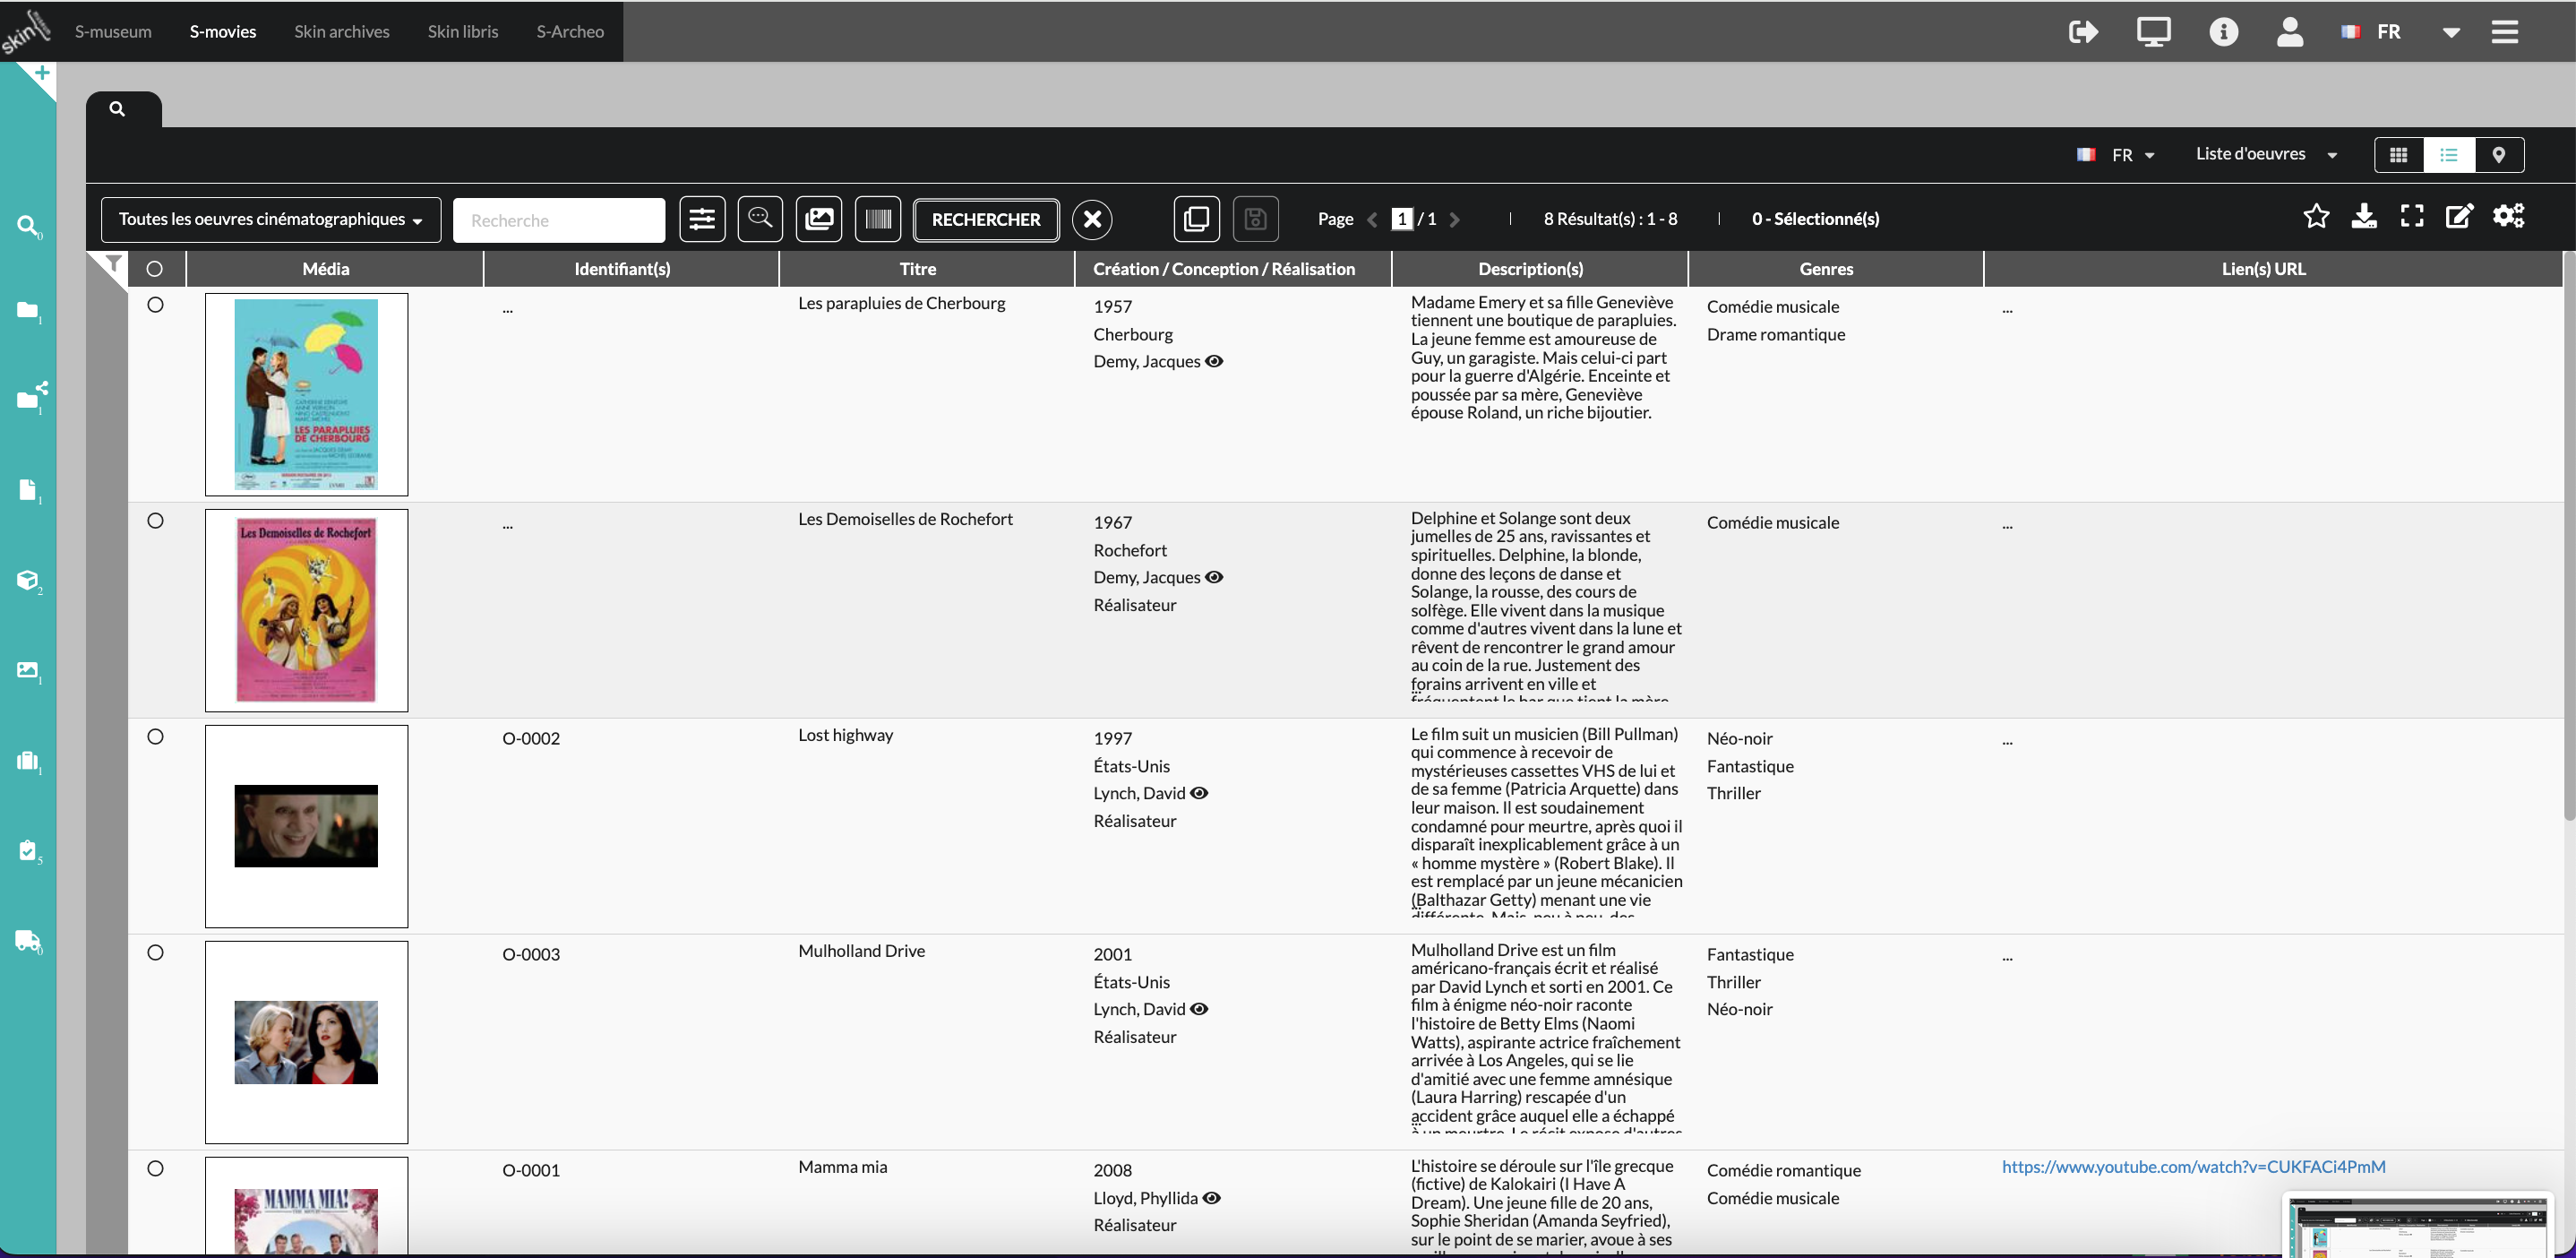
\includegraphics[width=0.85\textwidth]{images/image.png} 
	
	\caption{Page d'accueil de l'espace de travail} 
	
	\label{figAccueil} 
	
\end{figure}

Une institution cliente de l’outil peut combiner un ou plusieurs espaces de travail, selon les données à gérer. Cette structure permet justement d’adapter l’interface à chaque type de collection géré : objets de collection de musée, collections archéologiques, collections de films, collections bibliographiques, collections d’archives, etc. Chaque espace de travail permet notamment la gestion des acquisitions, des collections, de leurs mouvements, de projets, d’expositions, des médias... De plus, chaque espace de travail est structuré selon des normes de description et un cadre de modélisation adaptés au type de collection qui y est géré. L'espace de travail S-Movies est modélisé selon les préconisations de la FIAF sur l’adaptation du FRBR, et structuré selon les normes de descriptions évoquées. Ainsi, les collections sont organisées en trois entités distinctes, conformément aux adaptations du FRBR par la FIAF : Films, Manifestations, Œuvres cinématographiques (Films désigne ici le niveau Item), comme le montre la capture d'écran du menu de l'espace de travail, ci-dessous :   

\begin{figure}[htbp] 
	
	\centering 
	
	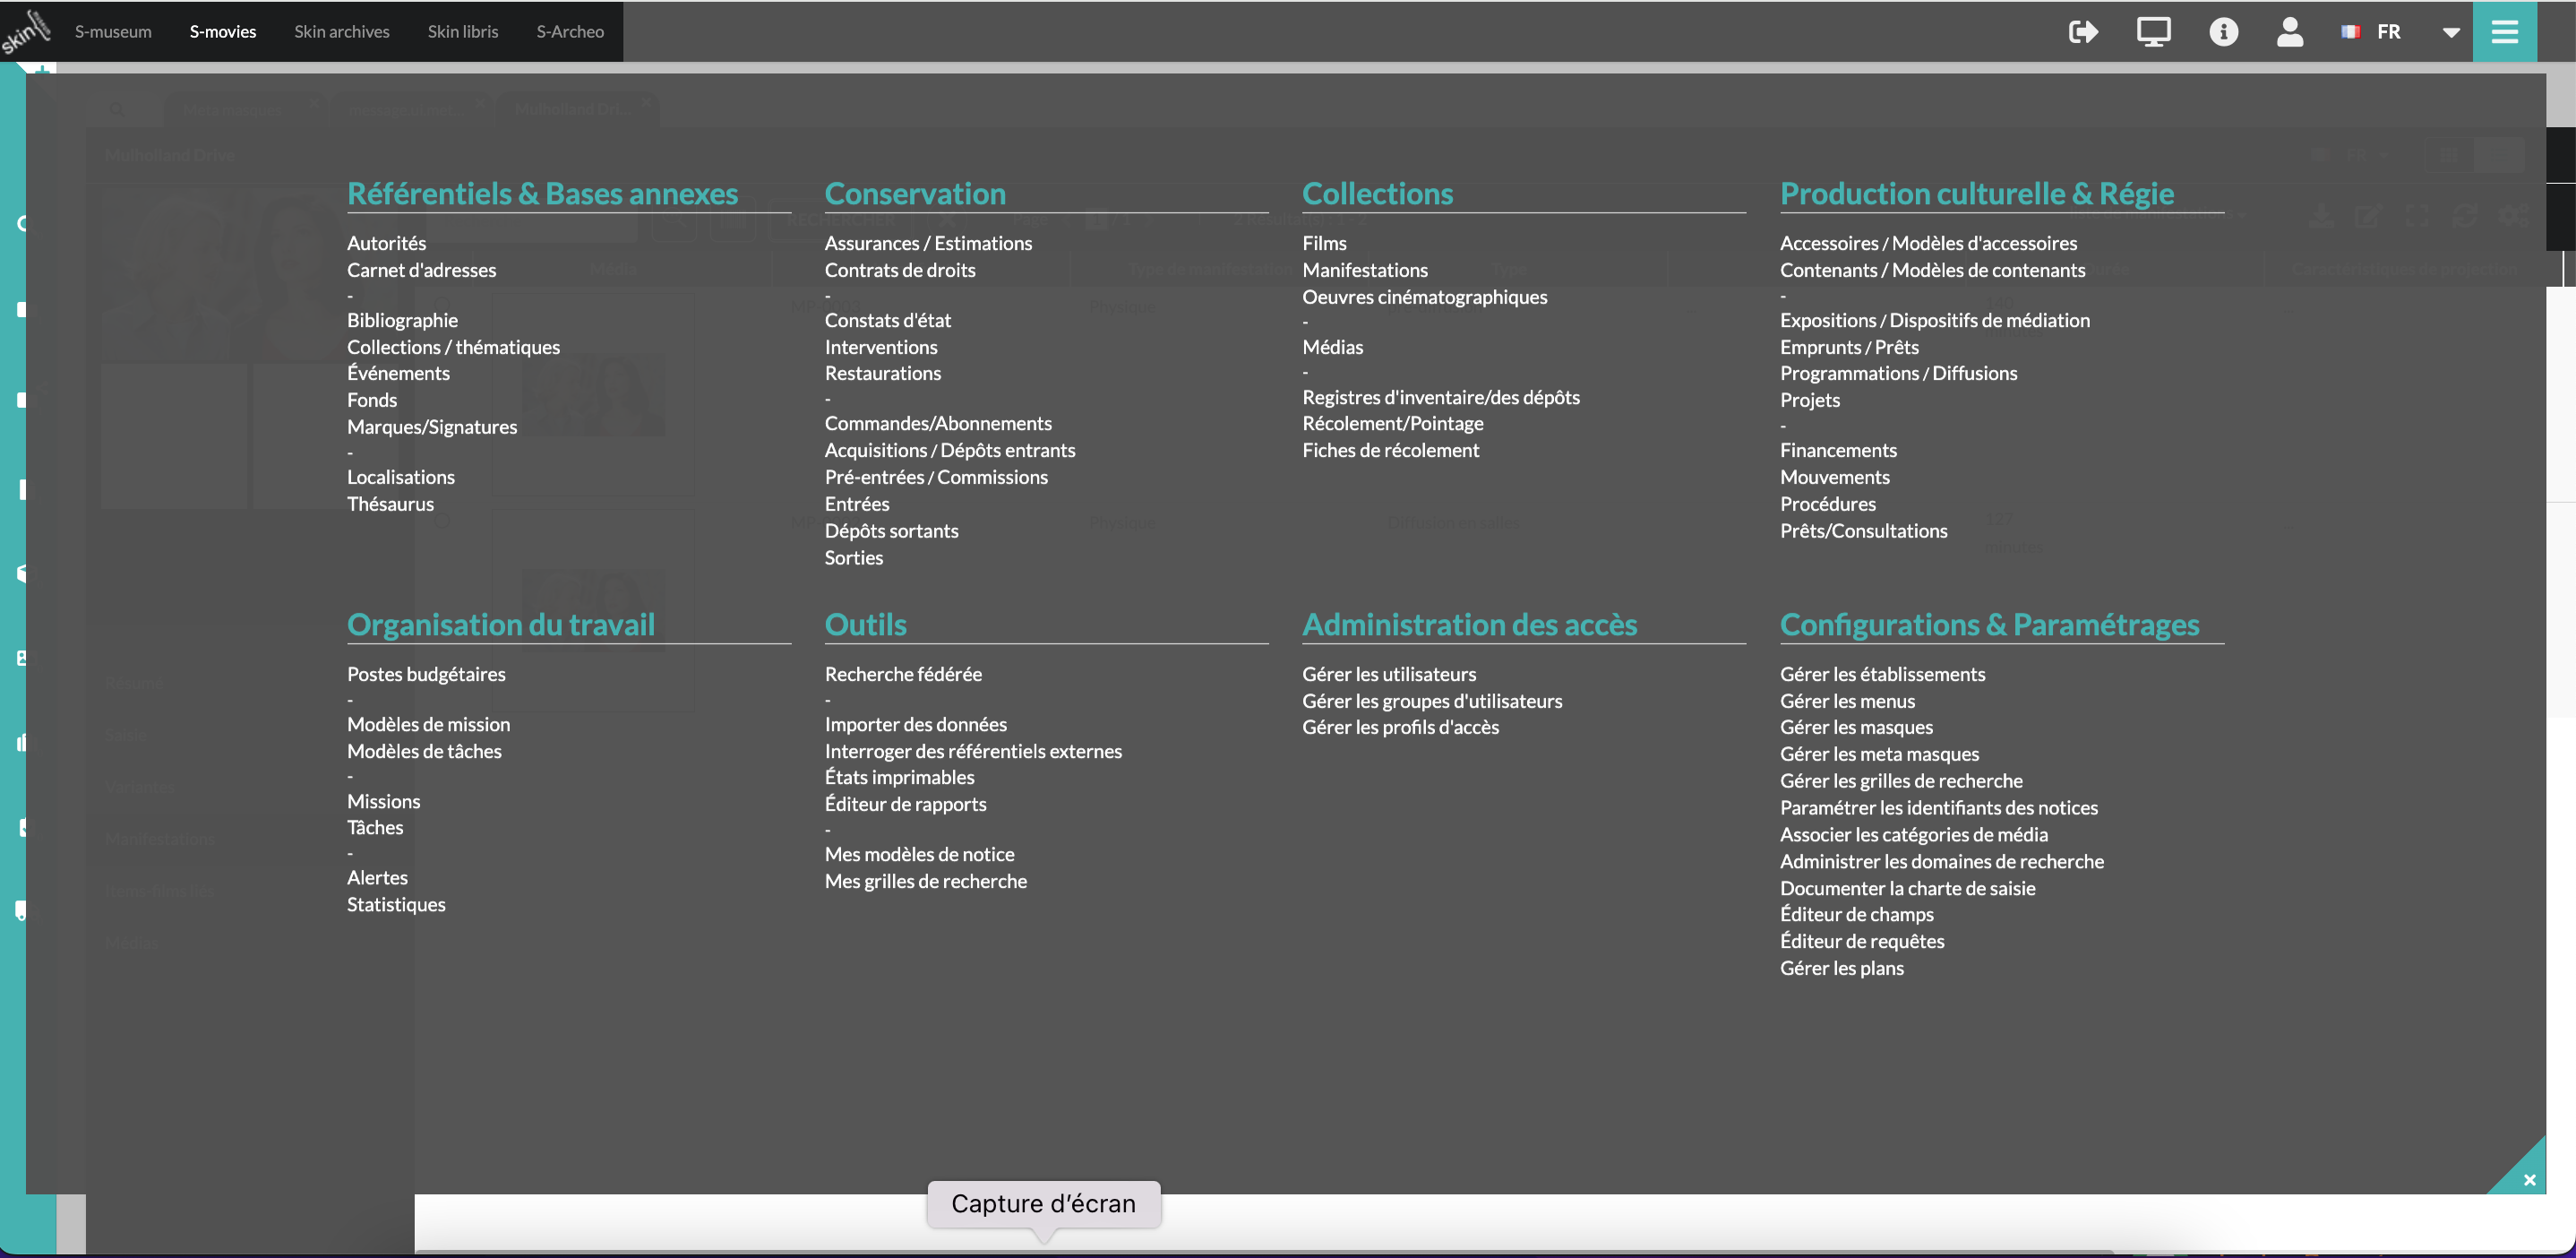
\includegraphics[width=0.85\textwidth]{images/image6.png} 
	
	\caption{Menu burger de l'espace de travail} 
	
	\label{figMenu} 
	
\end{figure}

Dans chacune de ces tables de données, l'utilisateur peut créer de nouvelles notices, et y associer des notices des autres tables. Par exemple, depuis la table Œuvres cinématographiques, l'utilisateur peut créer une notice d’Œuvre et y associer des notices de Manifestations et d'Items qui y sont directement liées. La Variante telle que définie dans le manuel de la FIAF n’est pas représentée par une entité à part entière sous la forme d’une table comme c’est le cas pour les autres entités. Toutefois, il est possible de créer une notice de Variante au sein de la table Œuvres cinématographiques, directement liée à une Œuvre. La Variante aura le même statut qu’une Oeuvre, mais elle sera de type Variante.  

Par exemple ci-dessous, une notice d’Œuvre cinématographique à laquelle sont associées deux notices de Manifestation :  

\begin{figure}[htbp] 
	
	\centering 
	
	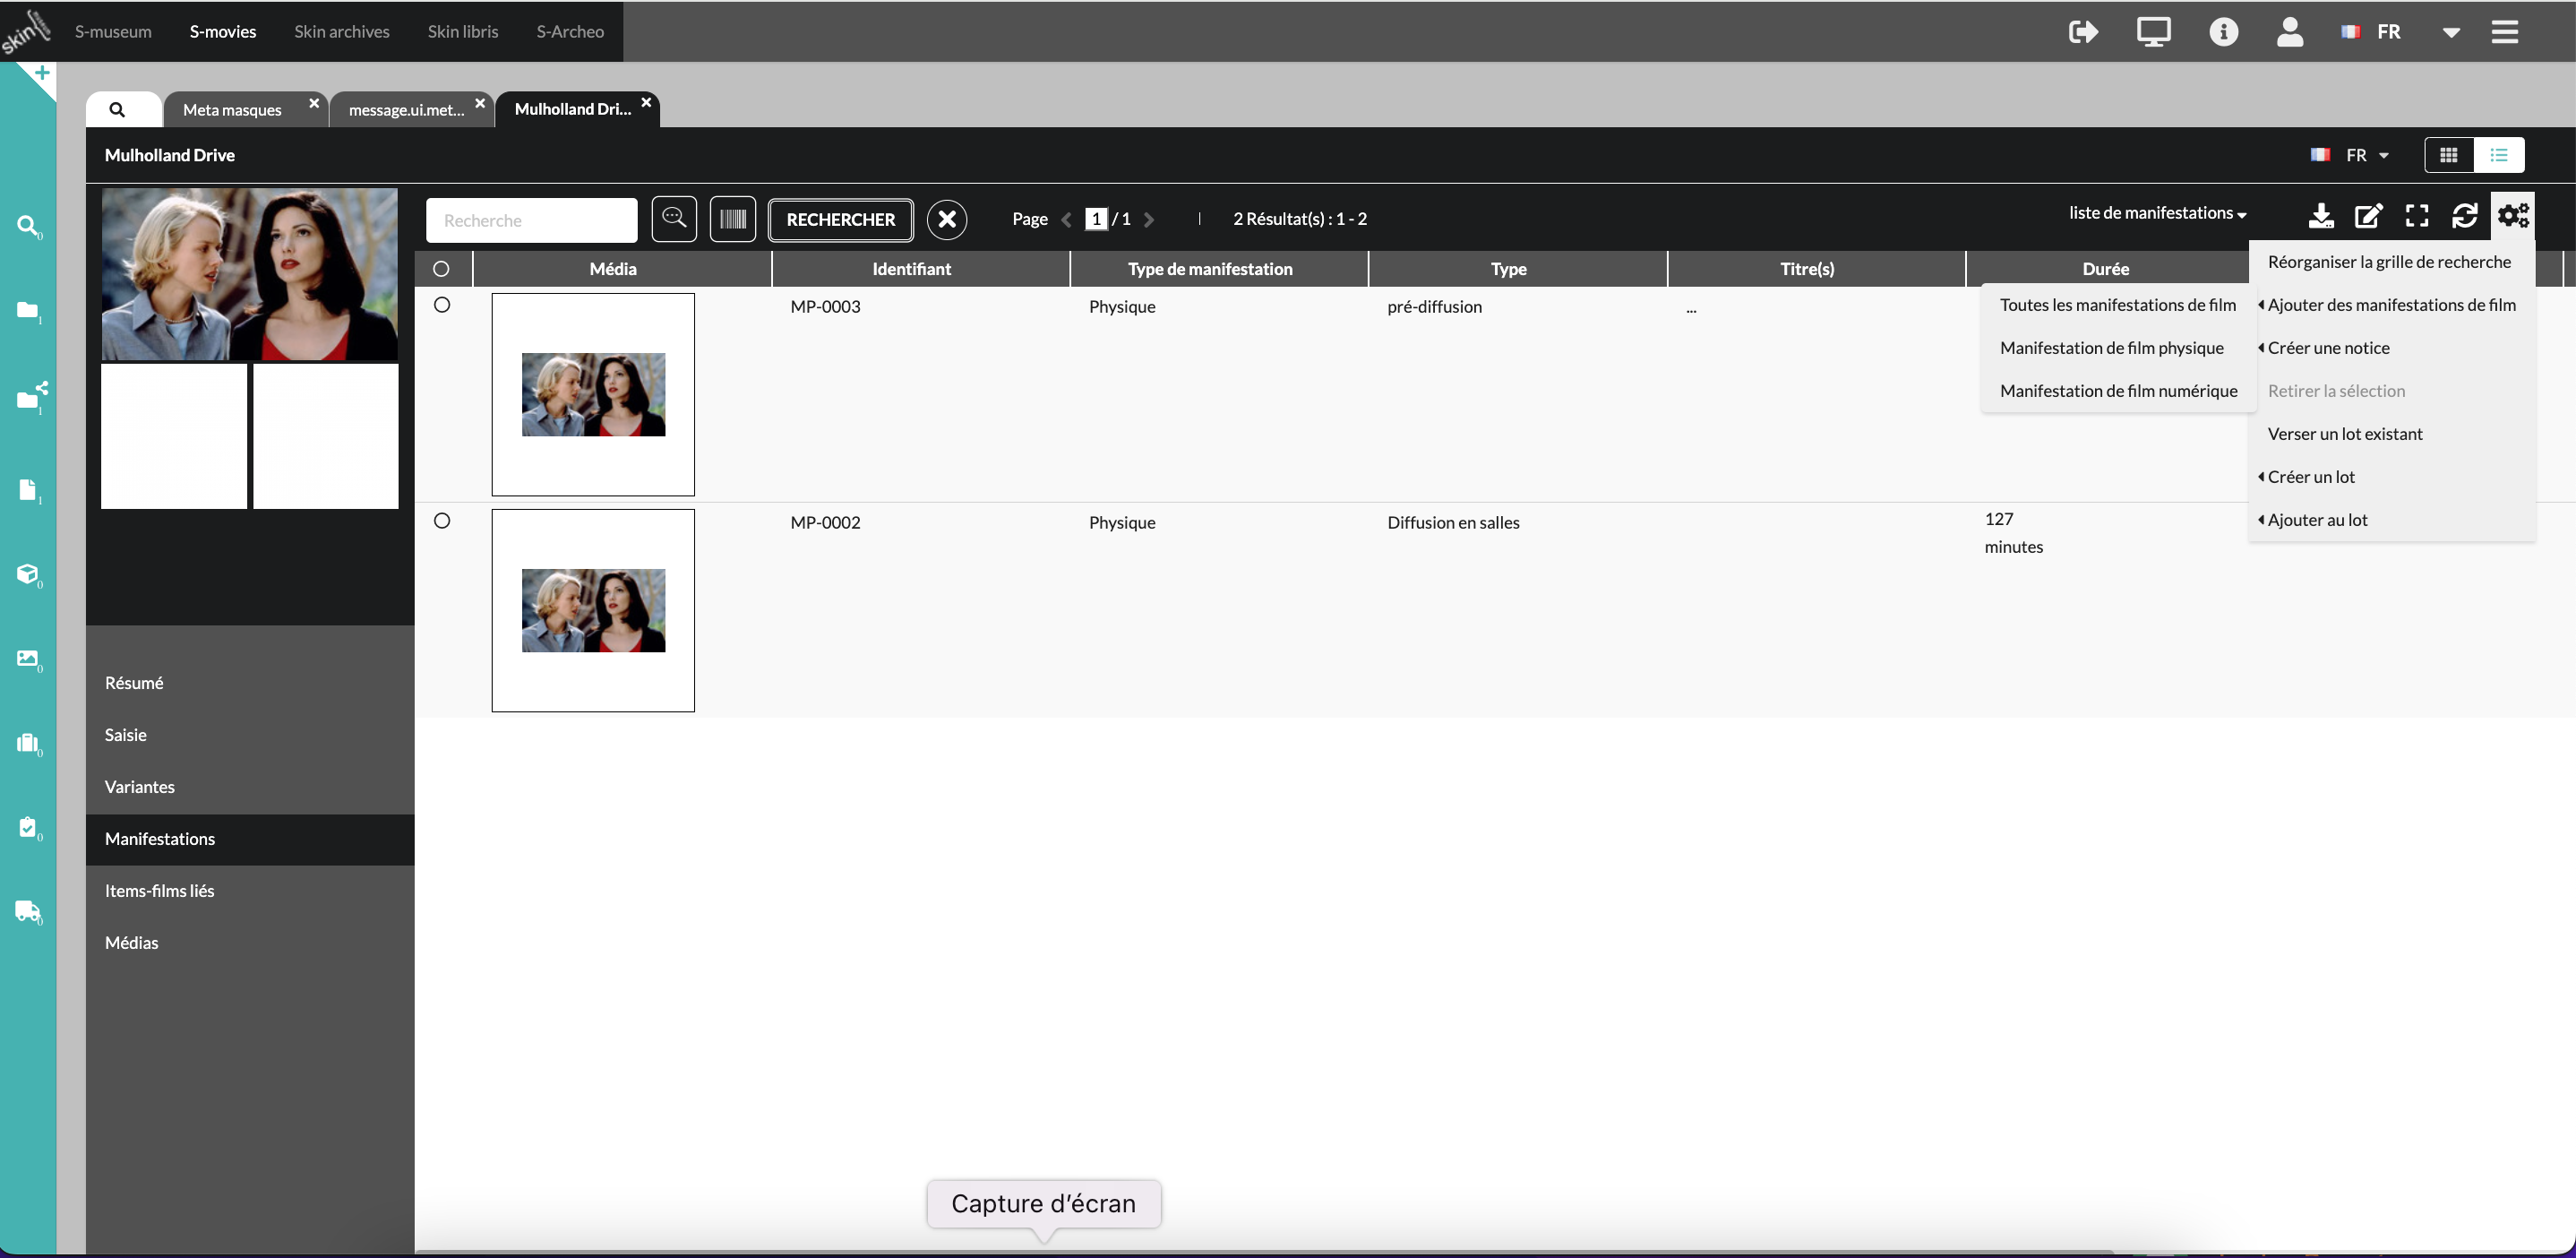
\includegraphics[width=1.0\textwidth]{images/image7.png} 
	
	\caption{Menu burger de l'espace de travail} 
	
	\label{figNoticeOeuvre} 
	
\end{figure}

L’interface permet d’associer des notices depuis un bouton d’action situé à droite.  

De plus, en fonction de la nature du corpus géré, un paramétrage adaptatif est prévu afin d’ajuster l’interface aux pratiques métier de chaque institution. En effet, une adaptation supplémentaire de la modélisation de données via la configuration flexible de chacun des espaces de travail. Trois configurations sont principalement possibles : le paramétrage de champs de saisie pour chaque type de notice, l'organisation de ces champs dans des grilles de résultats de recherche, et l'assemblage des champs et des grilles de recherche dans des menus navigables pour chaque type de notice. (Schémas explicatifs ?) Ce paramétrage concrétise la modélisation de données selon le cadre de référence utilisé.  

%quel rôle joue la modélisation dans ce cas ? En amont du paramétrage ? Ou en aval ? (Reprendre la définition) ou tout ce paramétrage fait partie de la modélisation  

Ainsi, une double adaptabilité est proposée : d’une part un espace dédié à un type de collection et structuré en fonction des normes de description et de la modélisation de données préférée, et d’autre part un paramétrage précis de l’espace de travail, propre au type de corpus géré par l'institution cliente, concrétisant ainsi la modélisation de données propre qui sera utilisée.  

L’espace de travail S-Movies est pré structuré suivant la modélisation FRBR préconisée par la FIAF. Cette structure stable, permet à Skinsoft de proposer un espace de travail pré défini pour chaque institution préservatrice de ce type de collection. En revanche, les corpus audiovisuels préservés par différentes institutions peuvent être de toutes sortes, sur différentes thématiques, sous différents formats. Cette hétérogénéité suppose des règles métiers spécifiques, issues des besoins de gestion de la collection préservé. Ainsi, par exemple, une collection audiovisuelle expérimentale ou amateure ne nécessitera pas les mêmes champs de saisie, les mêmes thésaurus, ou de la même disposition des résultats de recherche, qu'une collection audiovisuelle industrielle, grand public.   

Concrètement, au sein de l’espace de travail, la description d’un élément s’effectue au sein de champs de saisie, sélectionnés de manière adaptée aux besoins de description de l’institution donnée. Ces champs, s'ils sont paramétrables individuellement, font en réalité partie d'une structure plus large, à l'échelle de l'espace de travail dans lequel ils se situent. En effet, ces champs sont regroupés dans des masques, qui correspondent à des formulaires de saisie spécifiques au type de notice concerné. Par exemple, une notice de film physique, décrivant le niveau Item pourra contenir un masque de saisie, contenant des champs de saisie correspondants (cf \ref{figMasques}): identifiants, format de l’item, support de l’item, etc. 

\begin{figure}[htbp] 
	
	\centering 
	
	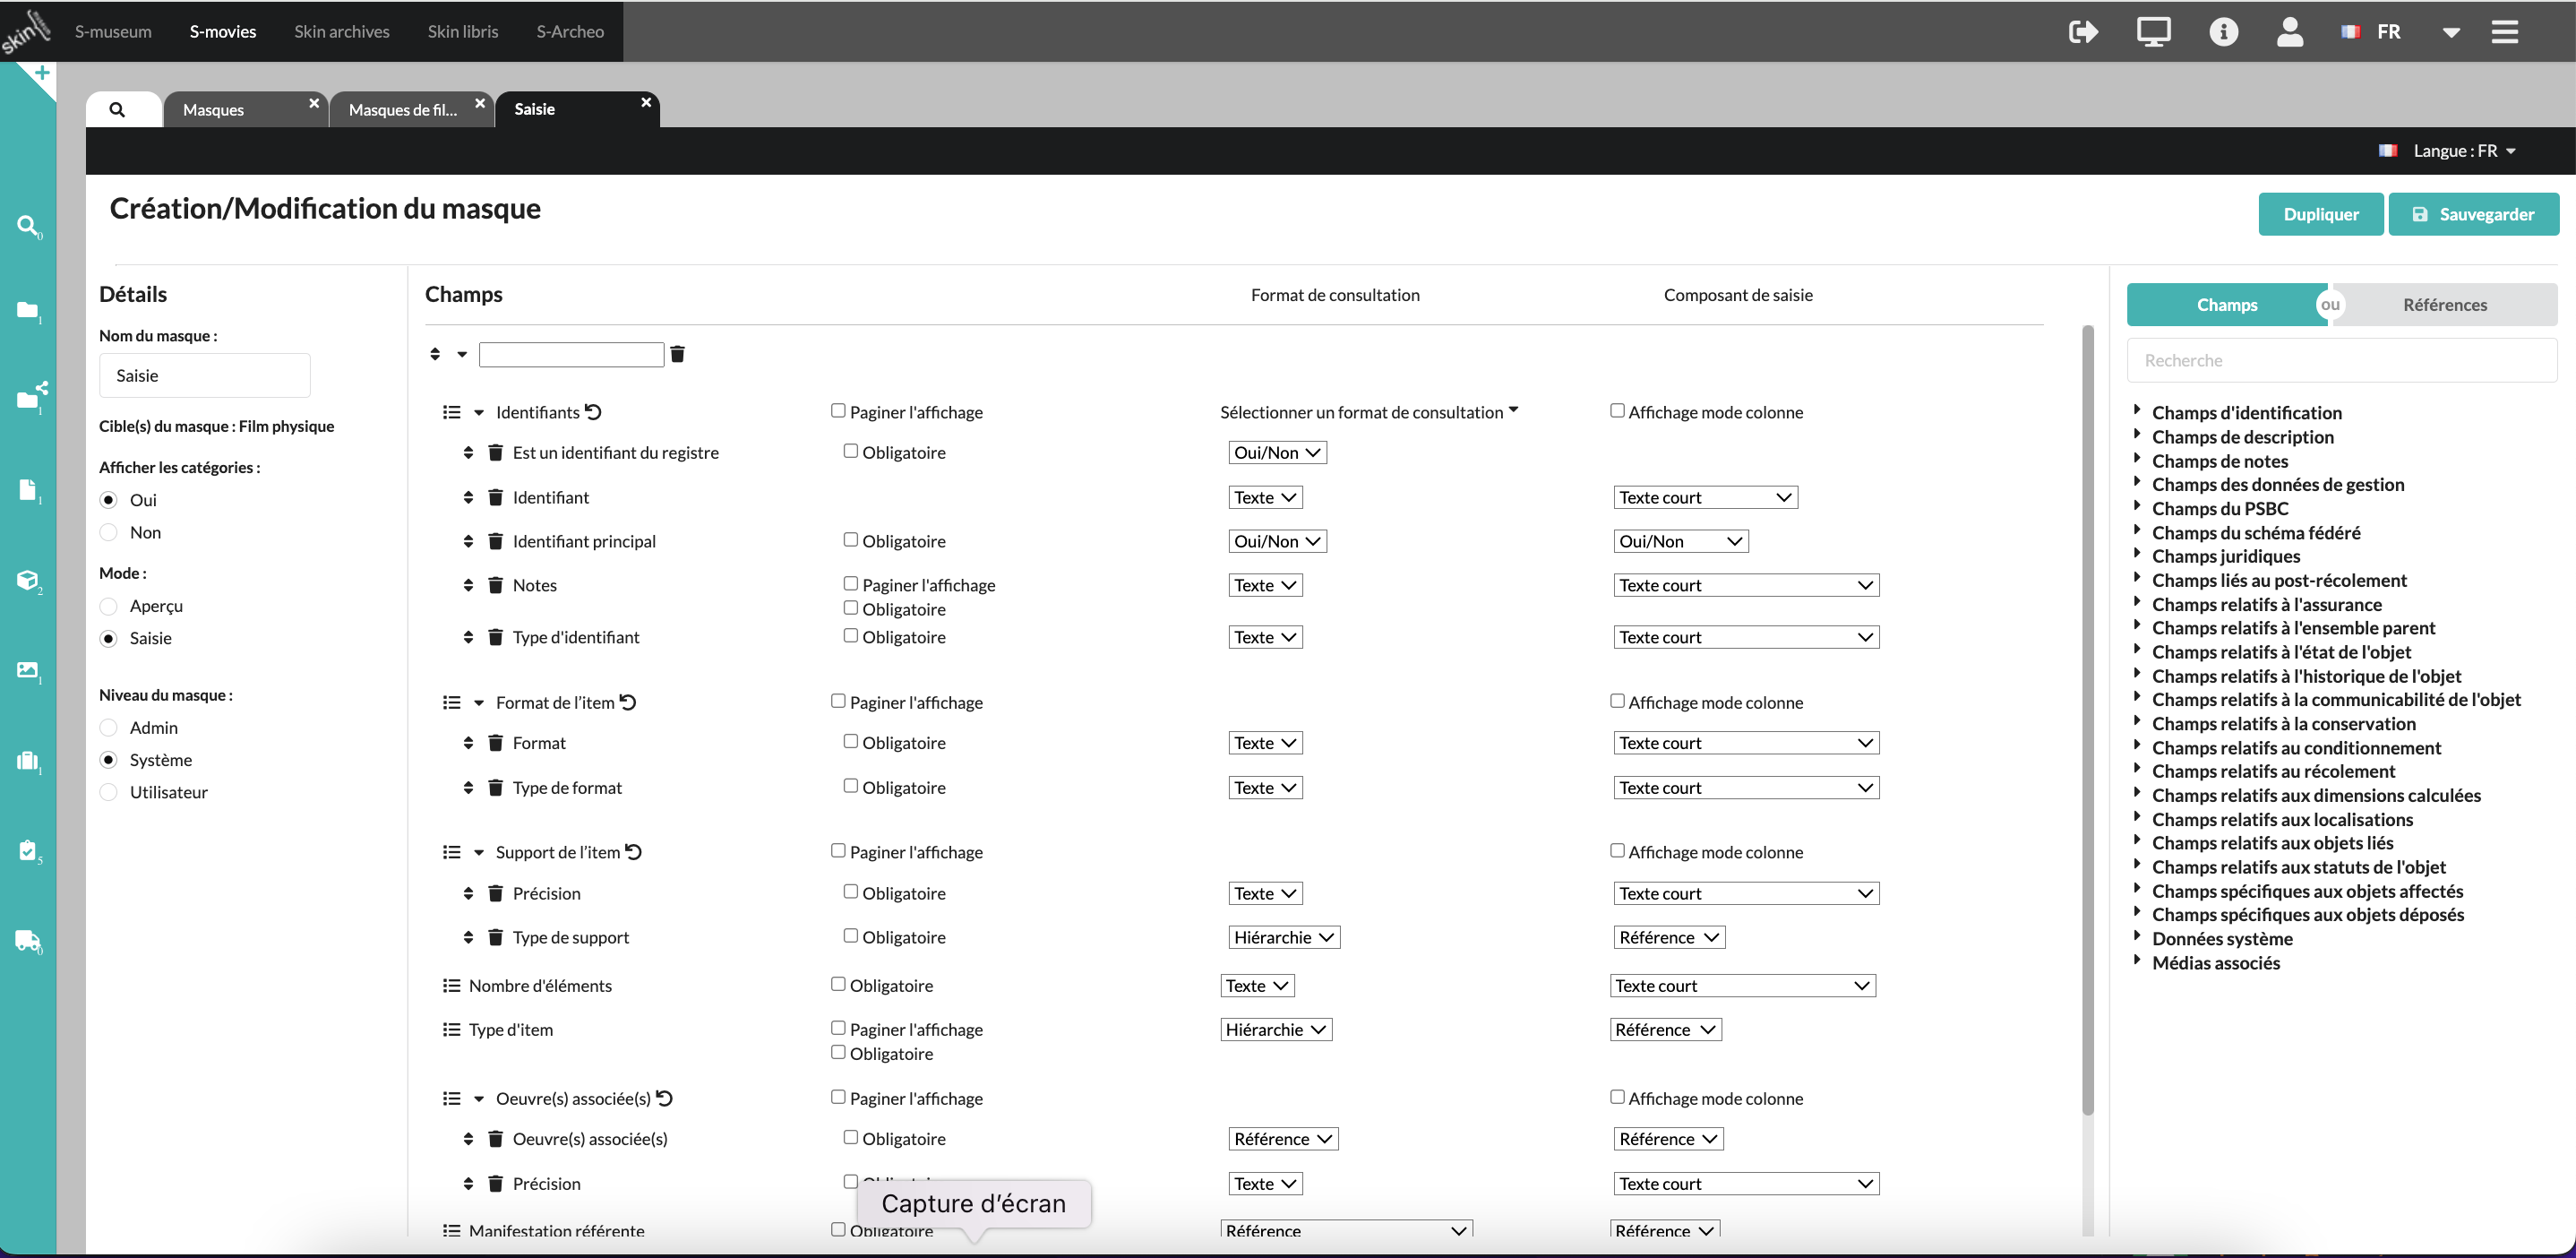
\includegraphics[width=1.0\textwidth]{images/image2.png} 
	
	\caption{Configuration des masques de saisie au niveau Item} 
	
	\label{figMasques} 
	
\end{figure}

Ce masque pourra ensuite être assemblé en tant qu’onglet au sein d’un menu d'une notice de film physique, permettant à l'utilisateur d'y remplir les champs que nous avons mentionnés. Ici, le menu d’une notice de film physique qui contient le masque de saisie mentionné plus haut :  

\begin{figure}[htbp] 
	
	\centering 
	
	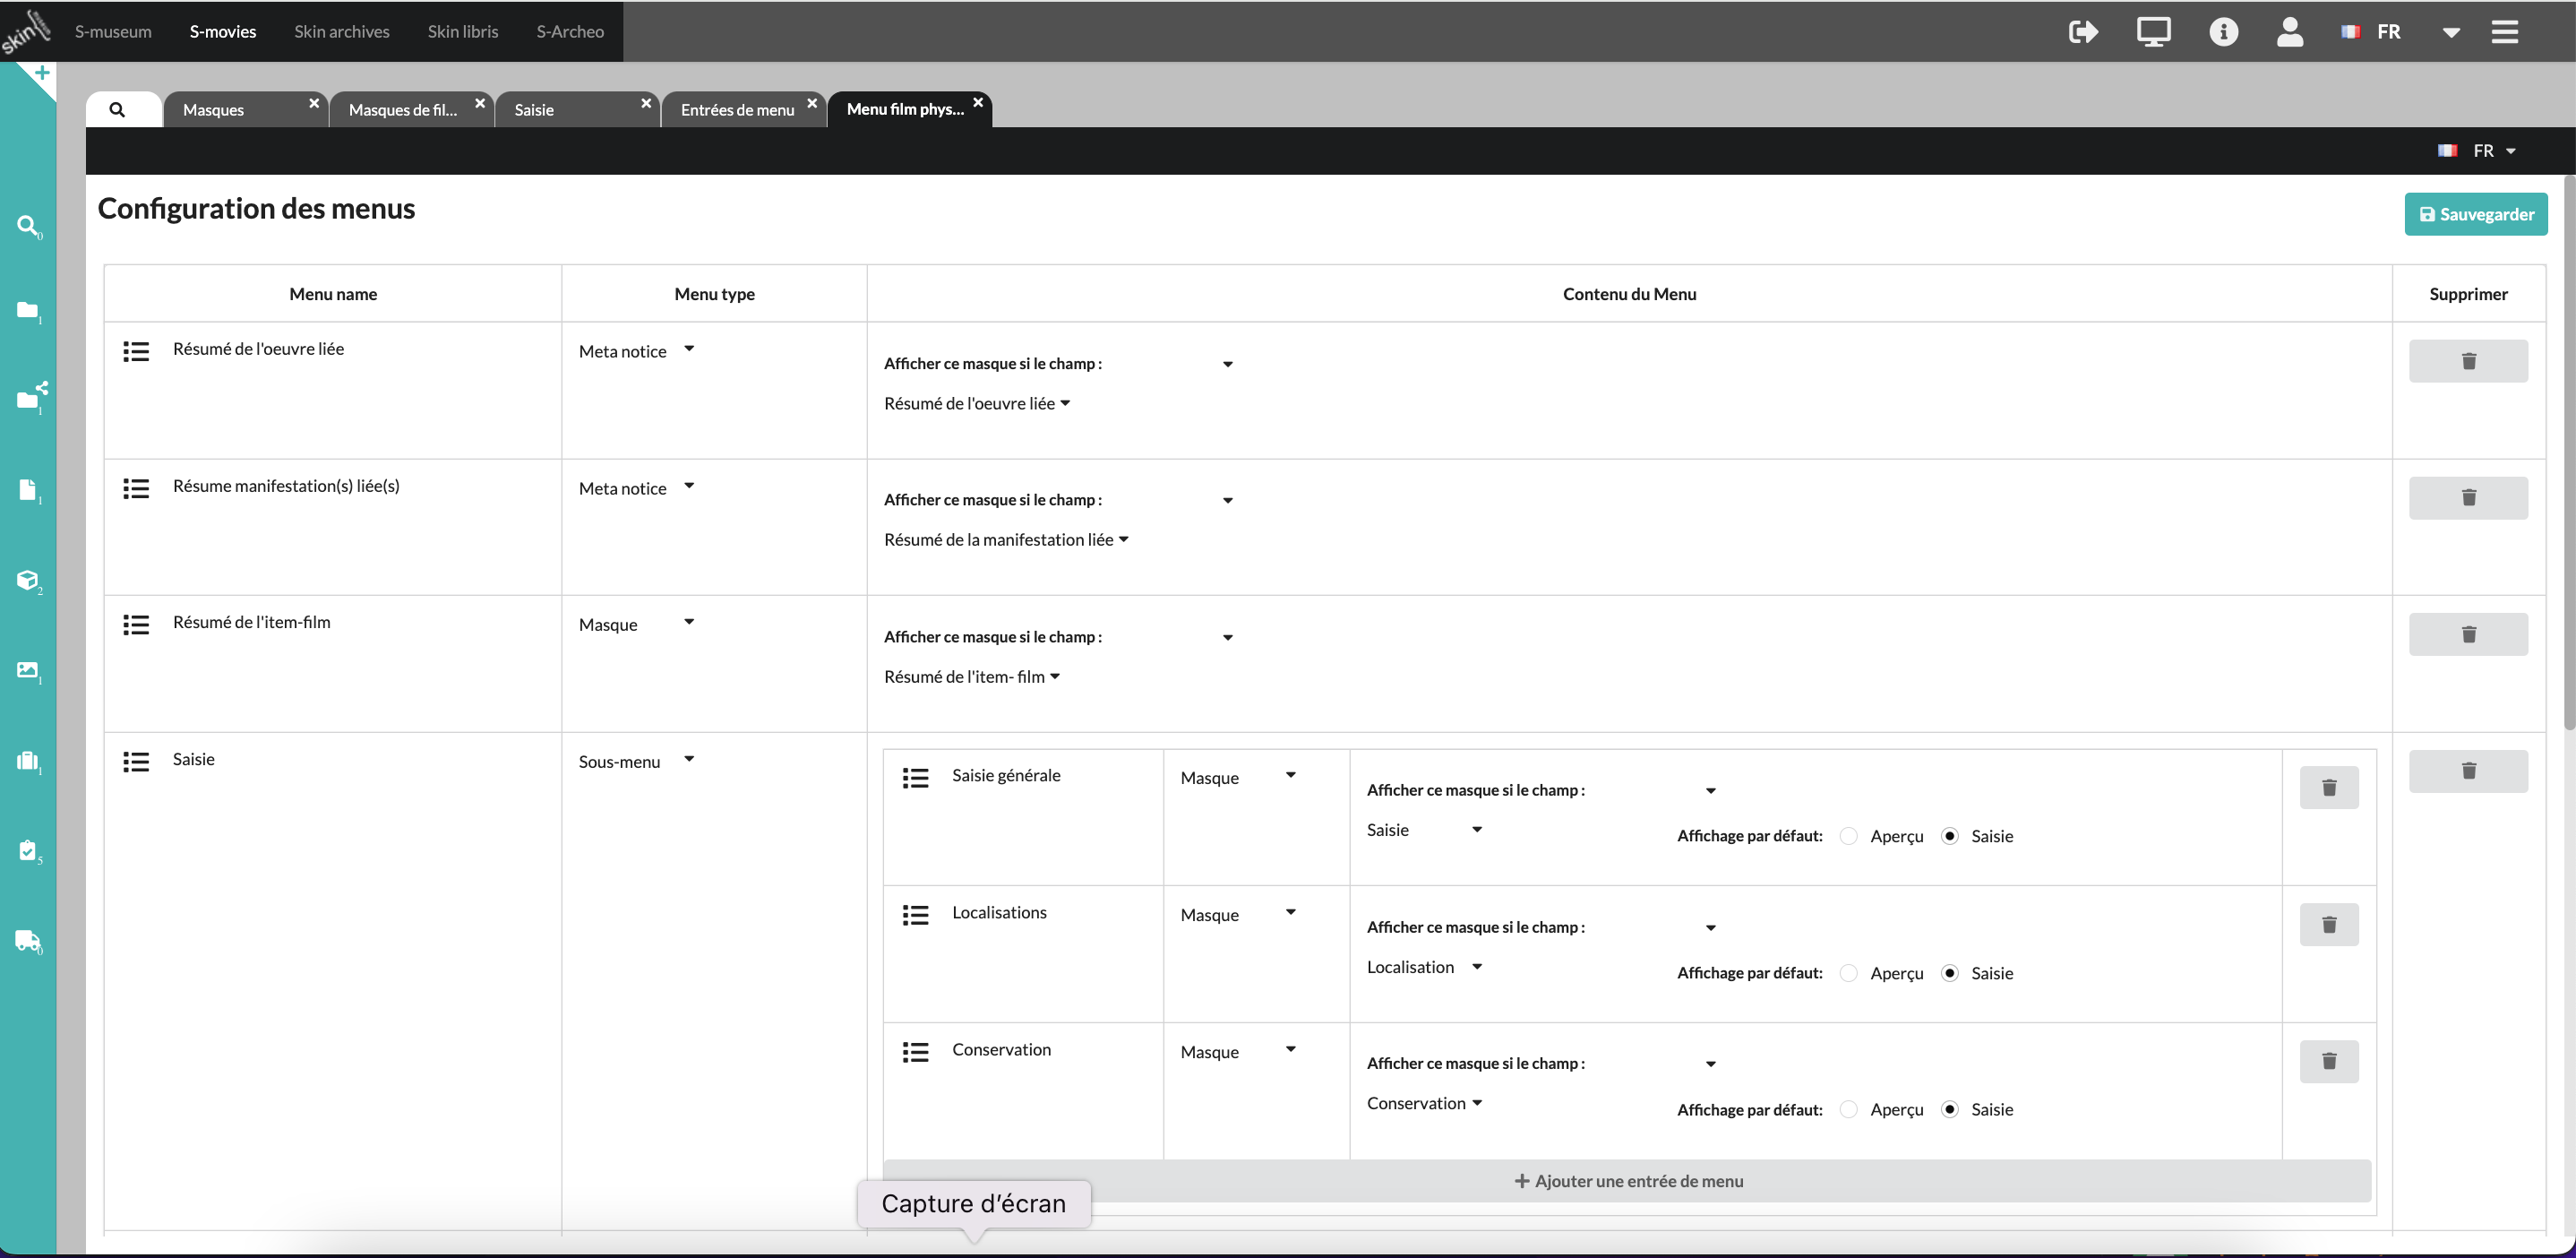
\includegraphics[width=1.0\textwidth]{images/image3.png} 
	
	\caption{Configuration du menu d'une notice de film physique} 
	
	\label{figMenuFilm} 
	
\end{figure}

Et ici la manière dont il s’affiche pour l’utilisateur, à la saisie dans une nouvelle notice de film physique :  

\begin{figure}[htbp] 
	
	\centering 
	
	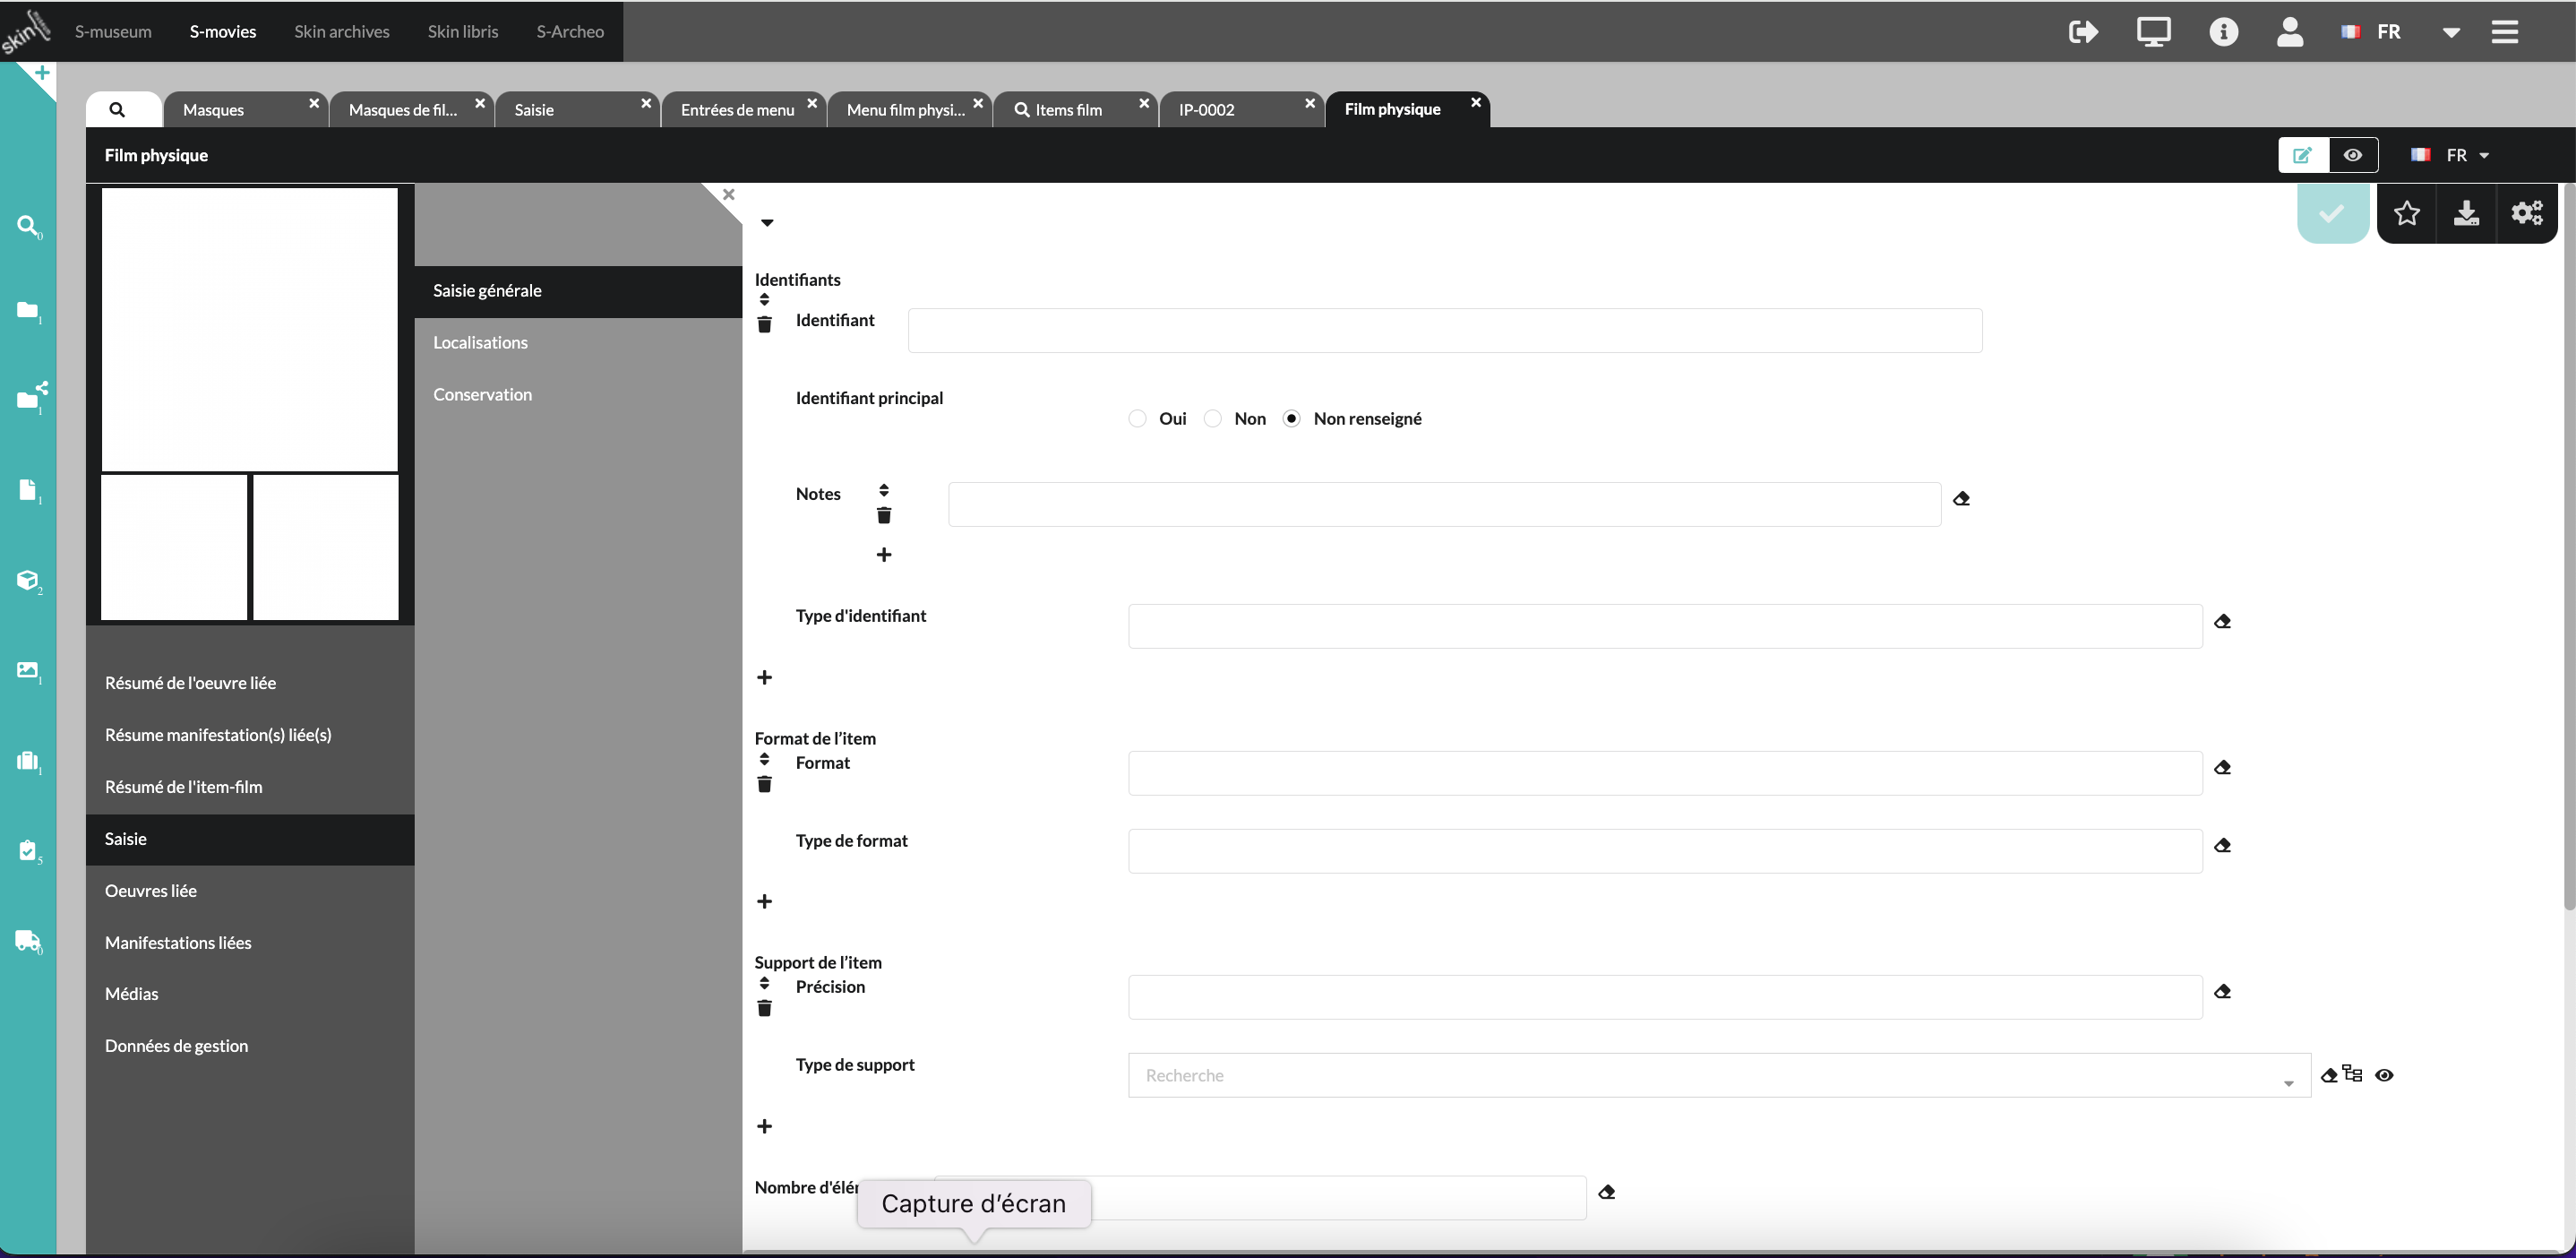
\includegraphics[width=1.0\textwidth]{images/image4.png} 
	
	\caption{Affichage du menu d'une notice de film physique à la saisie} 
	
	\label{figAffichageMenu} 
	
\end{figure}


Ce système d’organisation des masques de saisie au sein de menus permet également d’effectuer des liens avec d’autres types de notices et donc d’autres entités du FRBR. Par exemple la capture d'écran suivante \ref{figMenuGrilles}, montre que dans un menu de film physique, les onglets Œuvre liée et Manifestations liées permettent d’obtenir une grille de recherche, au sein d’une notice de film physique, affichant l’Oeuvre liée au film et les Manifestations dont il découle. 

\begin{figure}[htbp] 
	
	\centering 
	
	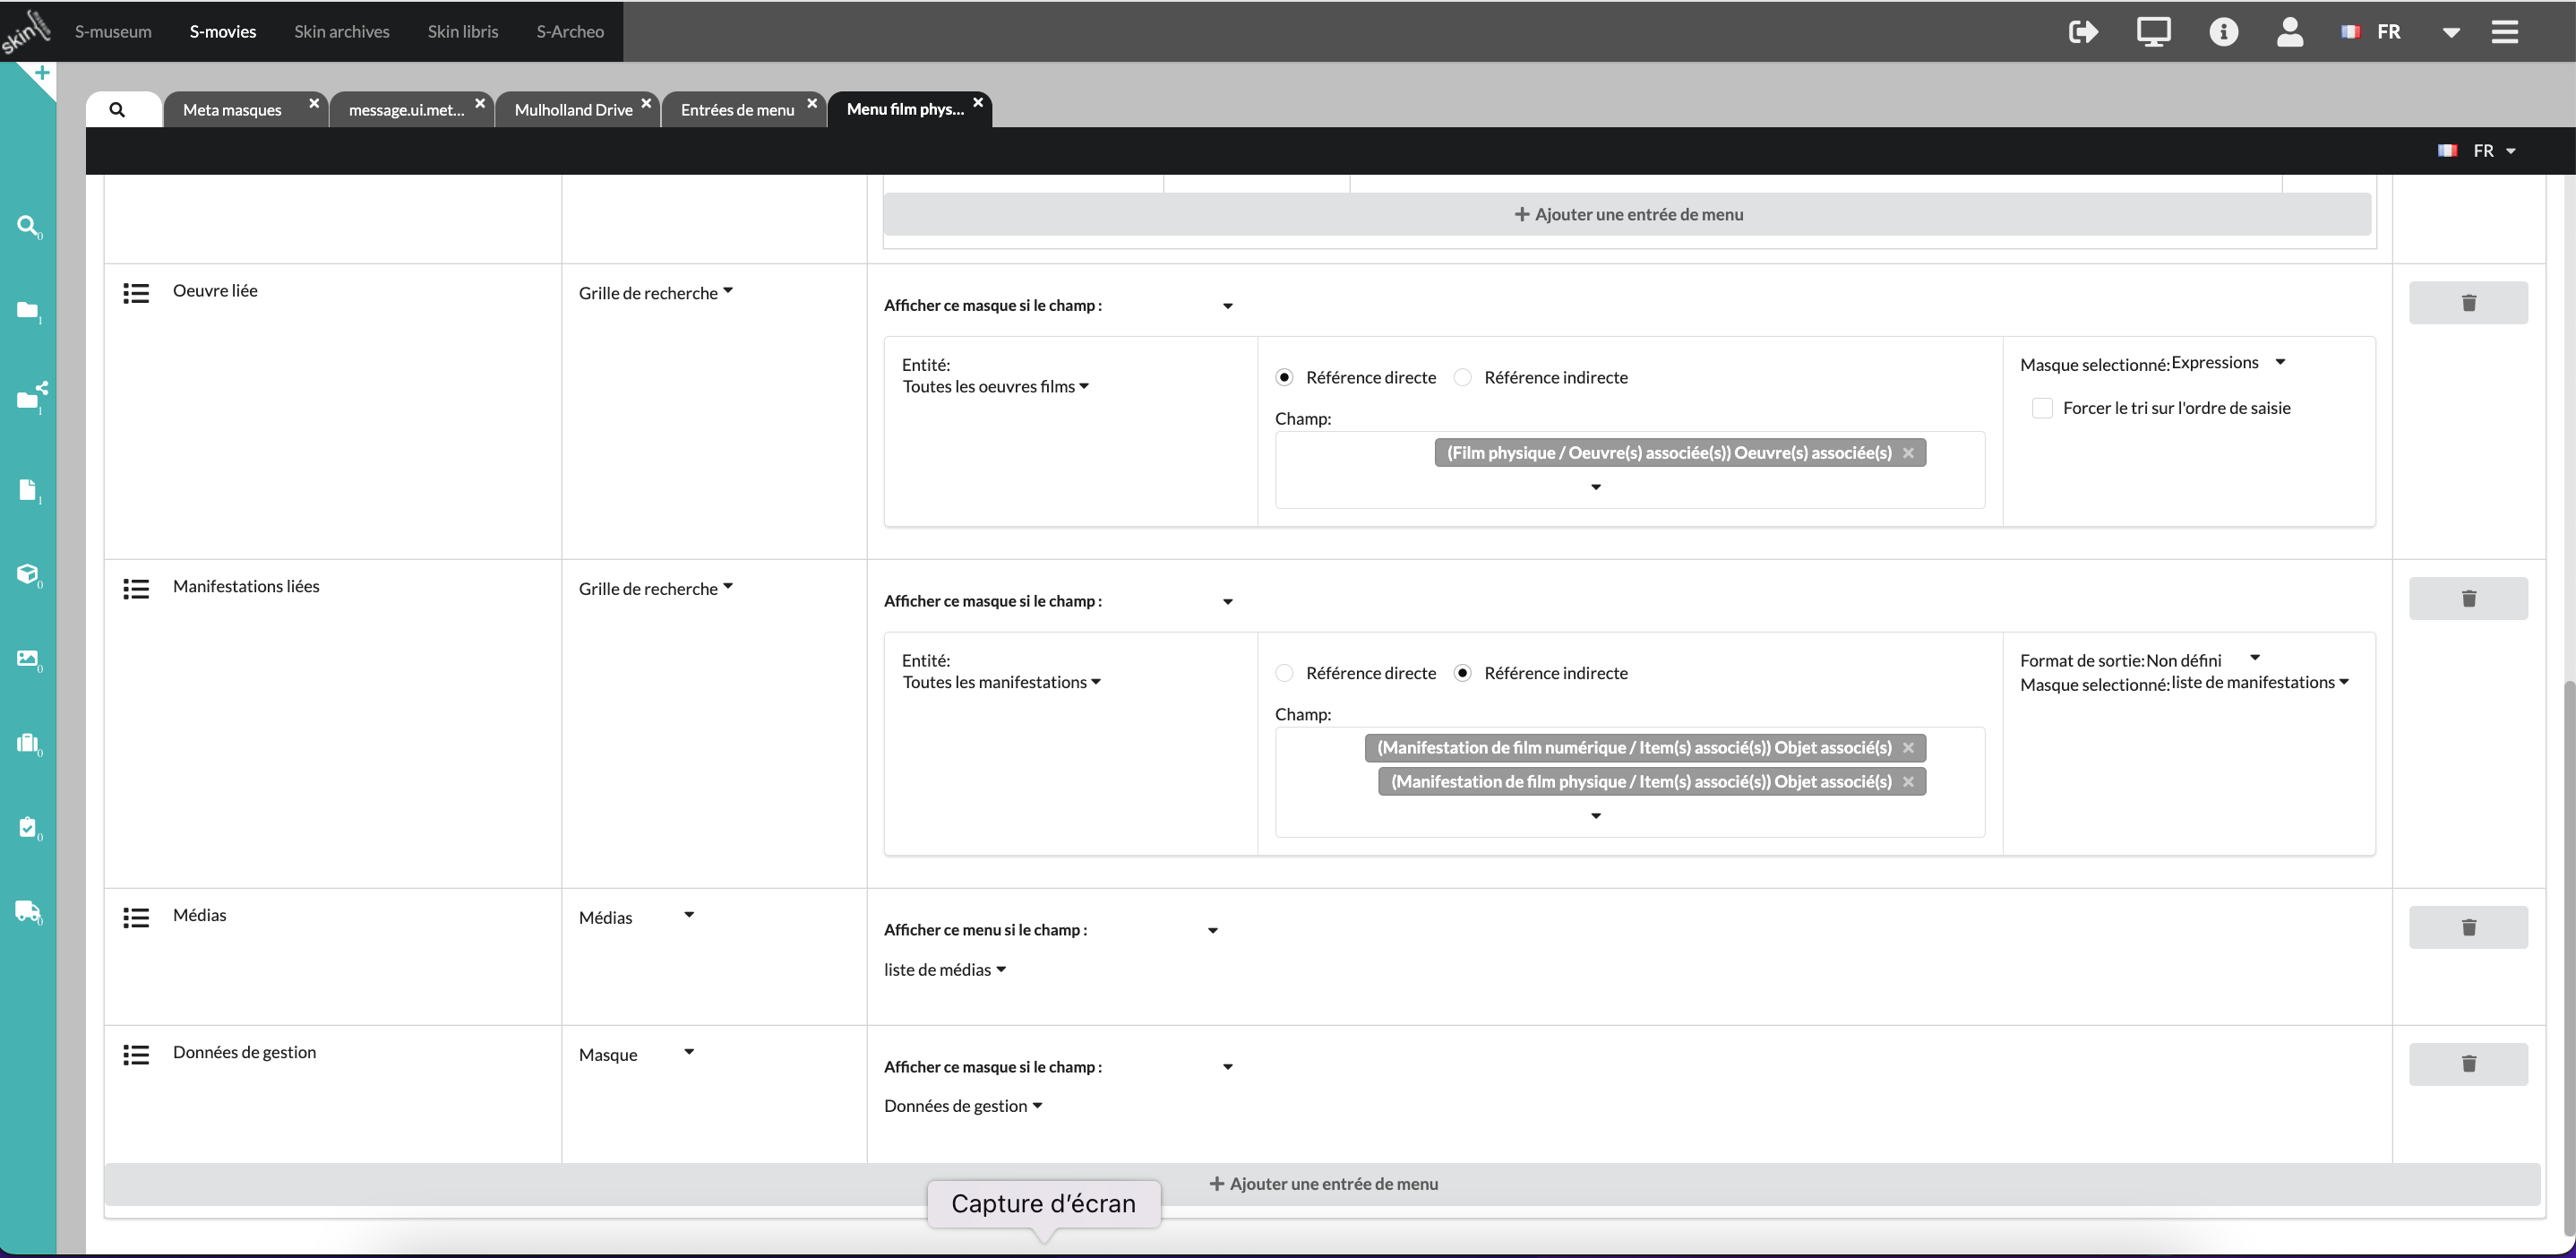
\includegraphics[width=1.0\textwidth]{images/image8.png} 
	
	\caption{Configuration de grilles de recherche pour l'affichage des éléments liés} 
	
	\label{figMenuGrilles} 
	
\end{figure}

L’affichage pour l’utilisateur au sein de la notice de film physique est le suivant, avec d’une part, l’Œuvre liée(\ref{figOeuvresLiées}, et d’autre part, les Manifestations liées \ref{figManifsLiées}: 

\begin{figure}[htbp] 
	
	\centering 
	
	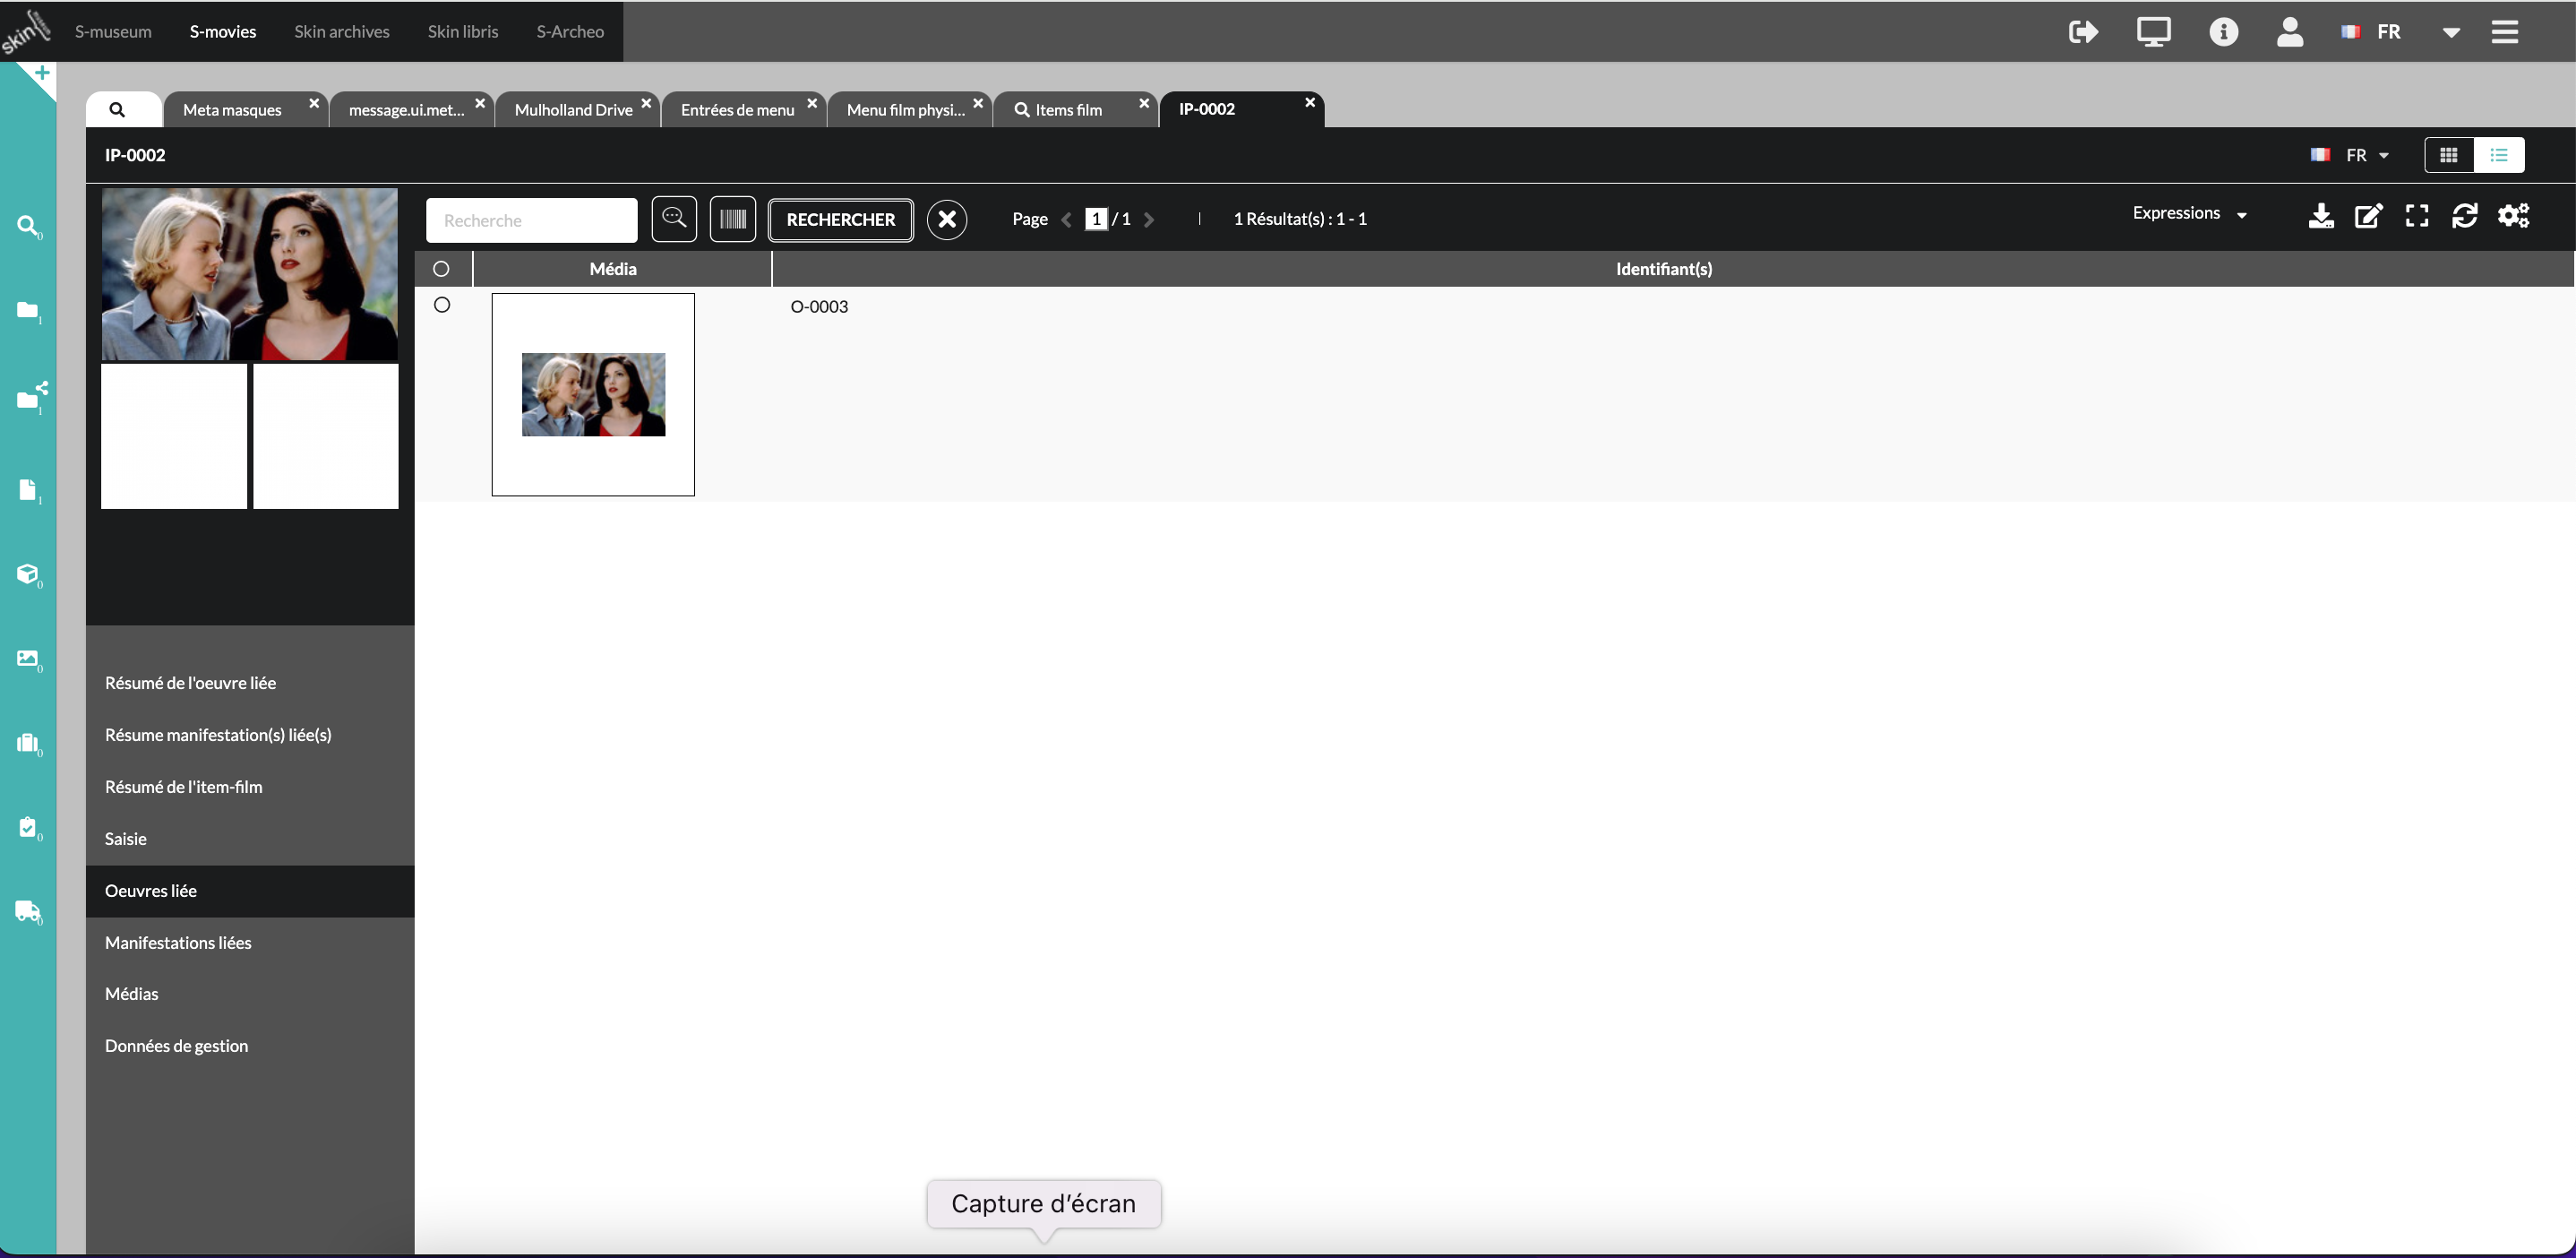
\includegraphics[width=1.0\textwidth]{images/image9.png} 
	
	\caption{Affichage des Oeuvres liées dans une notice d'item} 
	
	\label{figOeuvresLiées} 
	
\end{figure}

\begin{figure}[htbp] 
	
	\centering 
	
	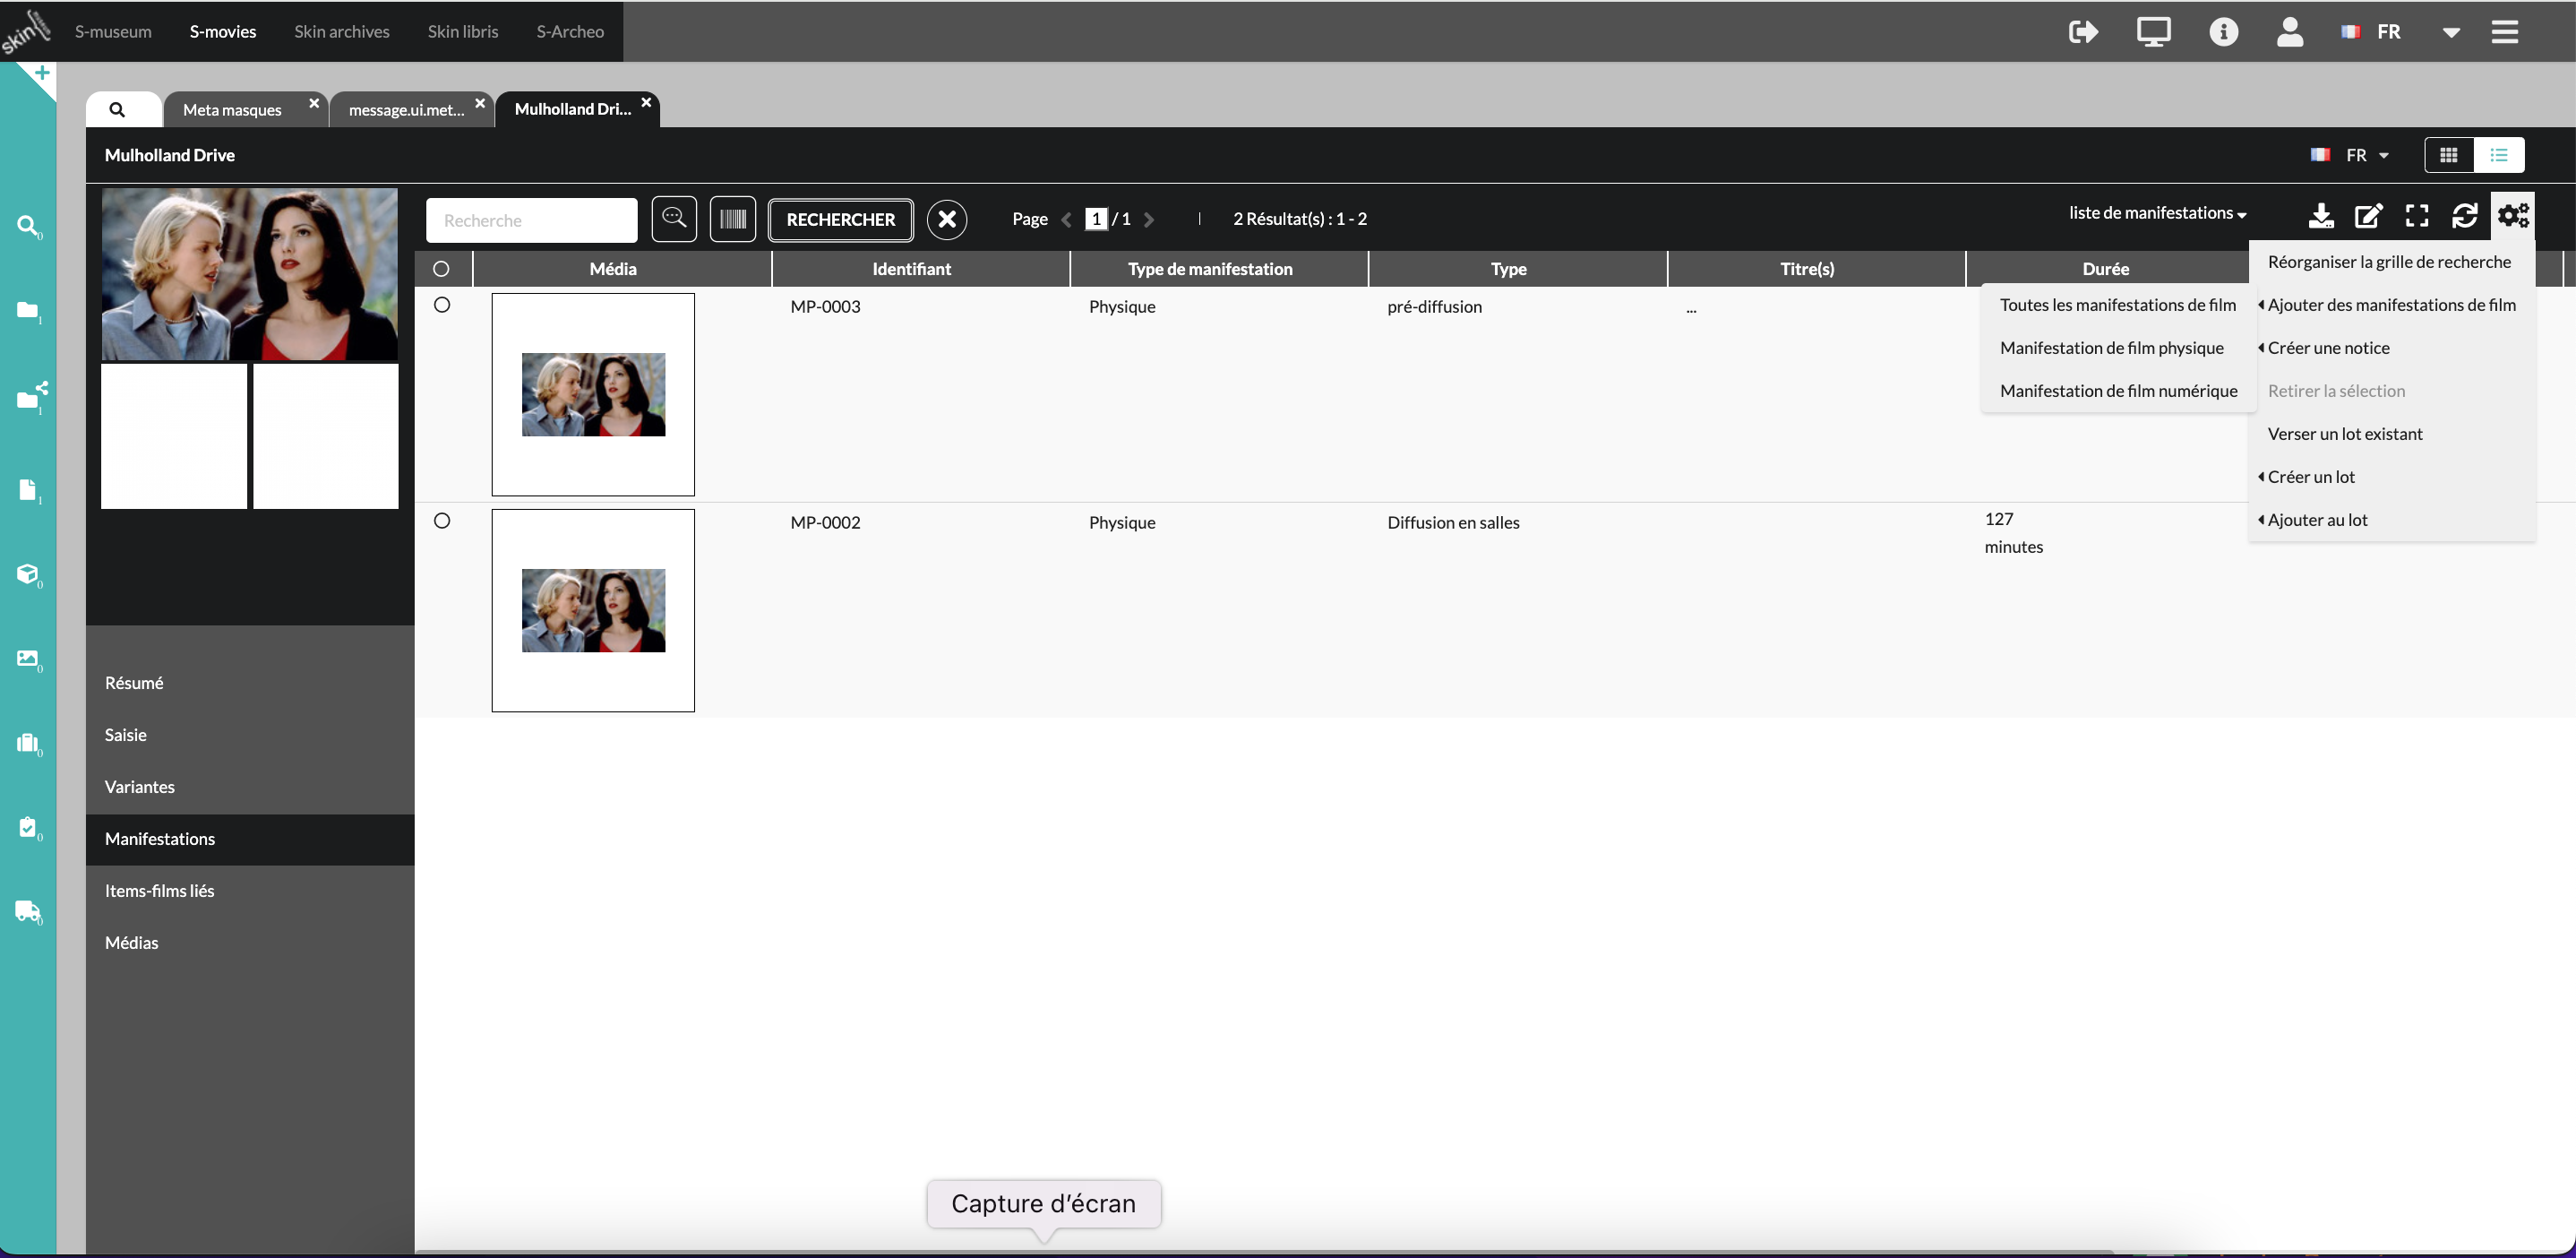
\includegraphics[width=1.0\textwidth]{images/image7.png} 
	
	\caption{Affichage des Manifestations liées dans une notice d'item} 
	
	\label{figManifsLiées} 
	
\end{figure}

Toutefois, les espaces de travail structurés sur le modèle FRBR, comme c'est le cas de S-Movies, requièrent un niveau de configuration supplémentaire, afin de concrétiser le découpage de la description en niveaux hiérarchiques. C'est le rôle des méta-masques, des formulaires de masques de saisie pouvant cibler les champs de plusieurs types de notices –et donc plusieurs niveaux du FRBR à la fois, afin d'imbriquer ces niveaux de description au sein d’une même notice. Ce système permet à l'utilisateur de saisir implicitement des éléments de description sur plusieurs niveaux du FRBR en une seule notice, permettant de surcroit au système de produire un héritage des champs d’un niveau à l’autre du FRBR.  

Concrètement, dans S-Movies, la notice d'Œuvre/Expression pointe sur les champs de l'Œuvre et de l'Expression, la notice de Manifestation pointe sur les champs de l'Œuvre, l'Expression et la Manifestation, la notice de l'Item pointe sur l'Œuvre, l'Expression, la Manifestation et l'Item. \textbf{(Faire un schéma explicatif) (citer le mode d'emploi interne ?)}. Ce mode de paramétrage de la description permet d’intégrer aux niveaux du FRBR inférieurs des champs hérités des niveaux supérieurs.  

\footnote{Notons que la présence du niveau Expression contredit le modèle FRBR préconisé par la FIAF, qui fusionne le niveau Expression dans celui d’Œuvre. Etant donné que Skinsoft possède d’autres espaces de travail modélisé sur le FRBR, comme c’est le cas de l’espace dédié à la gestion des collections bibliographiques, le niveau Expression existe seulement en théorie, mais inutilisé en pratique au sein de S-Movies.} 

Ici par exemple (\ref{figMetamasque}), un méta masque de saisie pour une notice de film physique, ciblé sur l’expression, le film physique, la manifestation de film physique, l’œuvre cinématographique : 

\begin{figure}[htbp] 
	
	\centering 
	
	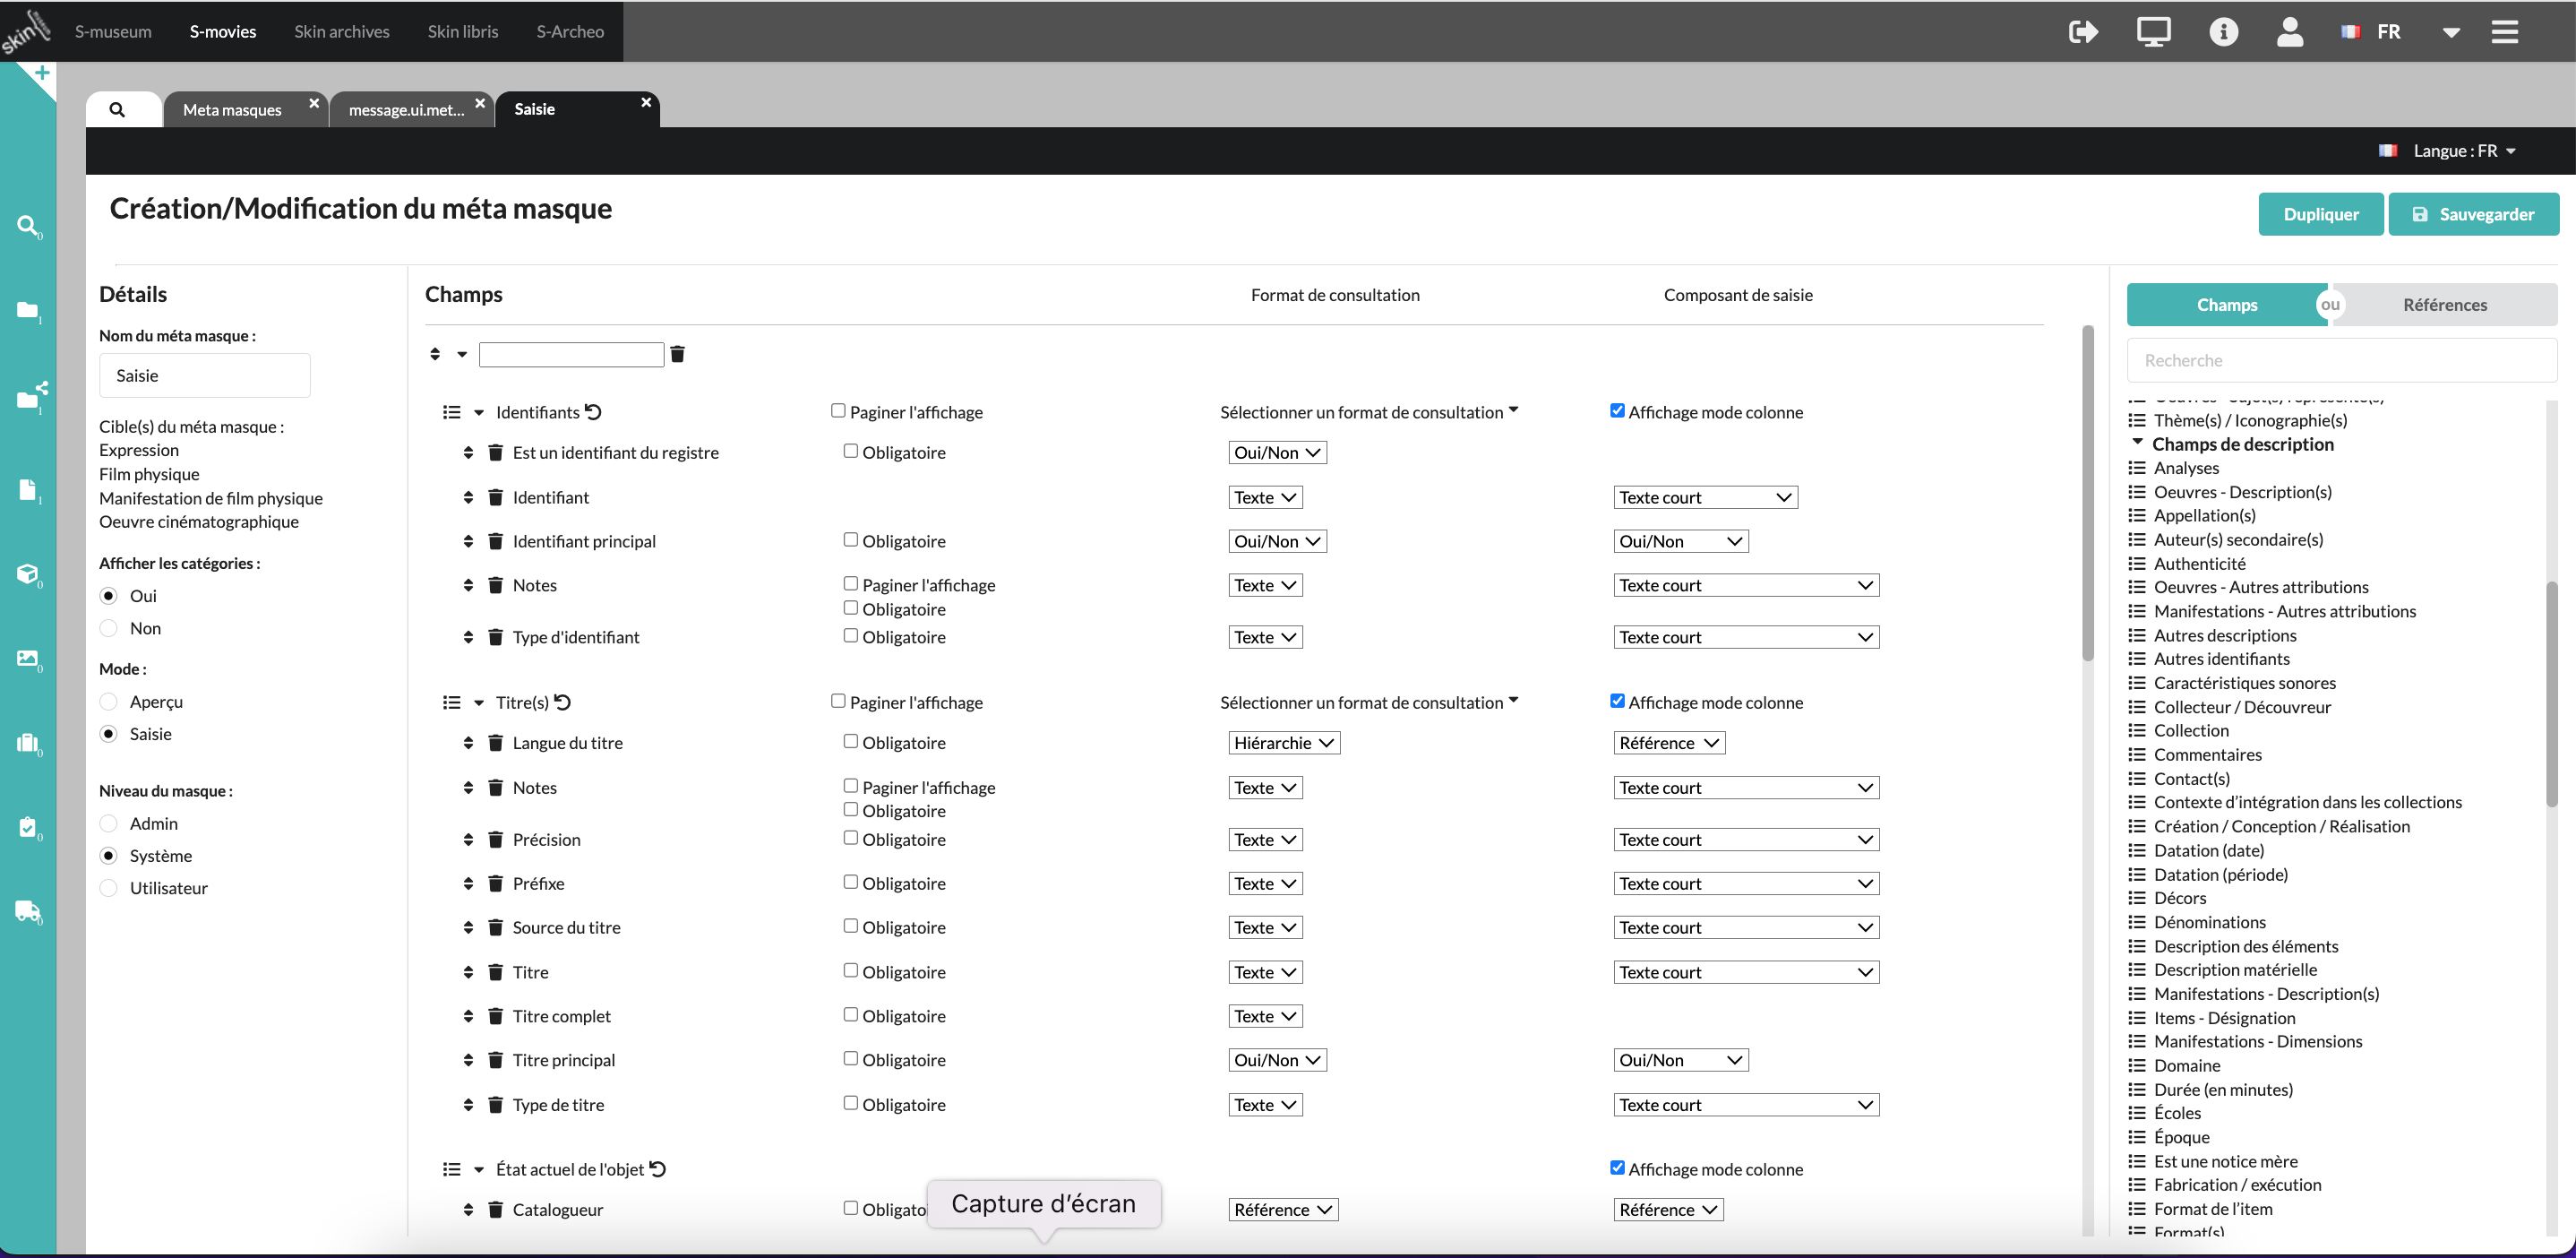
\includegraphics[width=1.0\textwidth]{images/imageb.png} 
	
	\caption{Configuration d'un méta-masque au niveau Item} 
	
	\label{figMetamasque} 
	
\end{figure}

À droite, les champs disponibles signalent à quel niveau de description ils appartiennent. Par exemple ci-dessus (\ref{figMetamasque}), le champ description appartient au niveau Œuvre, le champ dimensions appartient au niveau Manifestation.

%(: média (notice du fichier numérique, média), accessoire (modèle d'accessoire, accessoire), contenant (modèle de contenant, contenant).) 

Ces masques et méta masques créent ainsi une structure pérenne qui fait l'objet d'un paramétrage individuel qui permet d’ajuster la structure en fonction du type de collection et des usages métiers du client concerné. Ce paramétrage est défini au cours d’un travail de mapping entre les données client et la structure proposée par Skinsoft, afin de trouver un accord sur les champs qui seront utilisés pour la description des collections. L'équipe de Skinsoft organise ensuite ces champs dans des formulaires de saisie (masques et méta masques), eux-mêmes organisés pour constituer des menus de notice et des grilles de résultats de recherche. L'équipe produit également des imports de thésaurus propres aux usages de l'institution en question, afin d'assurer l'interopérabilité des données saisies. %Afin d'assurer l'interopérabilité des données, l'indexation des champs est liée à des thésaurus et des référentiels contrôlés qui ont importés au moment de la configuration de l'espace de travail pour le client. À développer  

Les fondements de l'architecture de S-Movies, doublement adaptée d’une part aux collections cinématographiques et d’autre part aux pratiques métiers spécifiques à chaque institution, constitue la condition de la qualité des données et de l’expérience utilisateur. L'enjeu de l'espace de travail est d'offrir une interface qui permette à l'utilisateur de décrire les collections en plusieurs niveaux sans difficulté et de pouvoir circuler entre ces niveaux et les liens qu’ils entretiennent. Cette circulation est notamment permise par les grilles de recherche que nous avons évoquées dont le paramétrage permet d’afficher les entités liées pour chaque notice. De plus, les différents outils de recherche permettent de circuler au sein des éléments de description indexés. (À développer ?) 

Toutefois, malgré la haute configurabilité de l’interface, l’hétérogénéité des corpus audiovisuels gérés d’une institution à l’autre complexifie le travail de mapping qui doit être effectué. En effet, la modélisation FRBR préconisée par la FIAF est un cadre qu’il s’agit d’ajuster aux pratiques spécifiques de gestion des collections, elles-mêmes adaptées au type de corpus géré. L’ajustement à des corpus audiovisuels spécifiques complexifie potentiellement la fluidité de la navigation entre les liens des différentes entités du FRBR au sein de l’interface.   

%Présentation espace S-Movies : aperçu des fonctionnalités communes et spécifiques (à placer en annexe ?): ces fonctionnalités sont chacune rattachées à un ou plusieurs niveaux du FRBR 

%- gestion des entrées : création d'un objet de collection via l'import de son média 

%- gestion des médias : associer un nouveau média à une notice de film ou un média existant 

%définir des vignettes sur les notices de films à l'aide des médias importés  

%- documents associés  

%- table collections/thématiques : regroupement des collections par thématiques : décrit le contexte de la collection, de l'assemblage des films, et présentent les items présents dans cette collection 

%- projets et mouvements : intervention, conservation, acquisitions, entrées, expositions, prêts, diffusion/programmation 

%fonctionnalités communes : gestion des contrats, évènements, interventions, expositions 

%Lien de la FIAF à S-Movies : mise en application du manuel de la FIAF, remodélisation, adaptable selon les corpus. tension public/privé 



%à bouger dans la première sous partie 

%S- Movies s'appuie sur deux normes descriptives audiovisuelles européennes : la norme EN 15744, qui définit le contenu obligatoire de description pour l'identification d'un film, ainsi que la norme EN 15907 qui découle du manuel de la FIAF et décrit une structure en couches et niveaux de données. Ces normes définissent les métadonnées essentielles pour faciliter l'échange de données et l'identification des films. \footcite{zotero-item-646} 



%Au niveau de la description des archives, il s'appuie sur la norme RDA pour la description et l'accès aux ressources. \footcite{zotero-item-646} 

%mentionner les données techniques ? : type de serveur, type de base de données 